\documentclass[sigconf]{acmart}
\setlength{\paperheight}{11in}
\setlength{\paperwidth}{8.5in}

\usepackage{fancyvrb}																				
\usepackage{hhline}
\usepackage{booktabs} % For formal tables
\usepackage{commentary-arxiv-private}
\usepackage{tabularx}
%\usepackage{sectsty}
\usepackage{titlecaps}
\usepackage{caption,subcaption}		

\usepackage{balance} % For balanced columns on the last page
\usepackage{booktabs} % For formal tables
\usepackage{amsmath}
\usepackage{graphicx}

\usepackage[linesnumbered,ruled,vlined]{algorithm2e}
\renewcommand{\algorithmcfname}{ALGORITHM}
\DefineVerbatimEnvironment{code}{Verbatim}{commandchars=\\\{\},frame=single,numbers=left,fontsize=\scriptsize}
\usepackage{paralist, tabularx}

\usepackage{epstopdf}
\usepackage{color}
\usepackage{url}
\usepackage{enumerate}
\usepackage[labelfont=bf]{caption}
\usepackage{xcolor}

% Template directives
\newcommand{\directive}[2]{%
	\ifx&#2&%
	\textbf{<\% #1 \%>}%
	\else%
	\textbf{<\% #1}{ #2 }\textbf{\%>}%
	\fi%
}


% Define our own compact enumerate
\newenvironment{compact_enum}
{\setlength{\leftmargini}{1em}
	\begin{enumerate}
		\setlength{\labelsep}{.3em}
		\setlength{\itemsep}{.4em}
		\setlength{\parskip}{0pt}
		\setlength{\parsep}{0pt}}
	{\end{enumerate}}

% Define our own compact itemize
\newenvironment{compact_item}
{\setlength{\leftmargini}{1em}
	\begin{itemize}
		\setlength{\labelsep}{.3em}
		\setlength{\itemsep}{.4em}
		\setlength{\parskip}{0pt}
		\setlength{\parsep}{0pt}}
	{\end{itemize}}

\newcommand{\gn}[1]  {\textit{#1}}              % (N)on-terminal
\newcommand{\gt}[1]  {\textbf{#1}}              % (T)erminal
\newcommand{\gl}[1]  {\texttt{\textbf{#1}}}     % (L)iteral
\newcommand{\gs}[1]  {\textit{#1}}              % (S)pecial construct
\newcommand{\gp}[0]  {$\rightarrow$}            % (P)roduction rule
\newcommand{\gd}[0]  { $|$ }                    % (D)isjunction


% Paths
\newcommand{\pp}[1]{\ensuremath{\hat{#1}}}
\newcommand{\contains}{\ensuremath{\supseteq}}

% Diffs
\newcommand{\diff}[3]{\ensuremath{\Delta^{#1}_{#2}(#3)}}
\newcommand{\insertarray}[1]{\diff{\operatorname{insert}}{\operatorname{array}}{#1}}
\newcommand{\insertbag}[1]{\diff{\operatorname{insert}}{\operatorname{bag}}{#1}}
\newcommand{\inserttuple}[1]{\diff{\operatorname{insert}}{\operatorname{tuple}}{#1}}
\newcommand{\append}[1]{\diff{\operatorname{append}}{\operatorname{array}}{#1}}
\newcommand{\update}[1]{\diff{\operatorname{update}}{}{#1}}
\newcommand{\delete}[1]{\diff{\operatorname{delete}}{}{#1}}
%\newcommand{\construct}[1]{\diff{\operatorname{construct}}{}{#1}}
%\newcommand{\destruct}[1]{\diff{\operatorname{destruct}}{}{#1}}
\newcommand{\construct}[1]{\diff{\operatorname{construct}}{\operatorname{unit}}{#1}}
\newcommand{\constructattach}[1]{\diff{\operatorname{construct\&attach}}{\operatorname{unit}}{#1}}
\newcommand{\destruct}[1]{\diff{\operatorname{destruct}}{\operatorname{unit}}{#1}}
\newcommand{\attach}[1]{\diff{\operatorname{attach}}{\operatorname{unit}}{#1}}
\newcommand{\detach}[1]{\diff{\operatorname{detach}}{\operatorname{unit}}{#1}}
\newcommand{\hpath}[1]{\ensuremath{\vec{#1}}}
\newcommand{\inserthtml}[1]{\diff{\operatorname{insert}}{\operatorname{html}}{#1}}
\newcommand{\appendhtml}[1]{\diff{\operatorname{append}}{\operatorname{html}}{#1}}
\newcommand{\updatehtml}[1]{\diff{\operatorname{update}}{\operatorname{html}}{#1}}
\newcommand{\deletehtml}[1]{\diff{\operatorname{delete}}{\operatorname{html}}{#1}}

\newcommand{\id}[1]{\hat{#1}}
\newcommand{\inst}[1]{I(#1)}
\newcommand{\diffz}[2]{\triangle^{\operatorname{#1}}(#2)}
\newcommand{\insertdiff}[1]{\diffz{insert}{#1}}
\newcommand{\inserttuplediff}[1]{\diffz{insert\_tuple}{#1}}
\newcommand{\insertarraydiff}[1]{\diffz{insert\_array}{#1}}
\newcommand{\appenddiff}[1]{\diffz{append}{#1}}
\newcommand{\attributediff}[1]{\diffz{attribute}{#1}}
\newcommand{\updatediff}[1]{\diffz{update}{#1}}
\newcommand{\deletediff}[1]{\diffz{delete}{#1}}

\newcommand{\highlight}[1]{\noindent\textbf{#1:}}

\def\env{\mathrm{\Gamma}}
\def\ground{\operatorname{Ground}}
\def\nav{\operatorname{Nav}}
\def\iterate{\operatorname{Iter}}
\def\outputarray{\operatorname{Out}^A}
\def\outputvalue{\operatorname{Out}^V}
\def\function{\operatorname{Func}}
\def\applyplan{\operatorname{Plan}}

% Definition environment
\newtheorem{base}{Base}[section]
\newtheorem{definition}[base]{Definition}
\newtheorem{example}[base]{Example}

% Tabular
\definecolor{lightgrey}{RGB}{235,235,235}
\definecolor{cream}{RGB}{255,255,204}
\newcommand\Tstrut{\rule{0pt}{2.6ex}}       % "top" strut
\newcommand\Bstrut{\rule[-0.9ex]{0pt}{0pt}} % "bottom" strut

% Copyright
%\setcopyright{none}
%\setcopyright{acmcopyright}
%\setcopyright{acmlicensed}
\setcopyright{rightsretained}
%\setcopyright{usgov}
%\setcopyright{usgovmixed}
%\setcopyright{cagov}
%\setcopyright{cagovmixed}


% DOI
\acmDOI{10.475/123_4}

% ISBN
\acmISBN{123-4567-24-567/08/06}

%Conference, May 14, 2017, Chicago, IL, USA

\acmConference[HILDA'18]{Workshop on Human-In-the-Loop Data Analytics}{June 2018}{Houston, TX, USA}
\acmYear{2018}
\copyrightyear{2018}

\acmPrice{15.00}

\newcommand{\projname}[0]{ViDeTTe}	
	

\begin{document}
\title{\projname\ Interactive Notebooks}

\author{Konstantinos Zarifis}
\orcid{1234-5678-9012}
\affiliation{%
  \institution{University of California, San Diego}
  %\streetaddress{P.O. Box 1212}
  %\city{Dublin}
  %\state{Ohio}
  %\postcode{43017-6221}
}
\email{zarifis@cs.ucsd.edu}



\begin{abstract}



\costas{high level comments I've addressed in our email exchange:\\
	* There isn't a clear vision of how the authors want notebooks to evolve: it just seems to be "Notebooks with embedded OLAP". That isn't carefully motivated in the paper, and arguably it's a bad idea. At some level, you're subverting the core UX idea of an electronic lab notebook as envisioned by Mathematica (and hence Jupyter). A lab notebook's role is to keep a record of a line of reasoning, so the scientist can revisit their process/thinking later, or share that process with others. Richly interactive interfaces--particularly ones that mutate "outputs"--in some sense abandon this goal. The result might be a terrific idea, or it might be an unnatural Frankenstein combination that is worse than the independent pieces. Do you have thoughts on this, and can you present arguments in your favor? In any case, you are moving notebooks closer to things like spreadsheets, web browsers and IDEs. You should think about whether your proposed user experience adds a useful point to the design space. \\
	-- Costas: Do you think that adding a ``Freeze" feature would be beneficial? This feature would "freeze" the displayed visualizations (and the interactive capabilities thereoff) so that no additional computation/ data access and redisplay will be triggered as a result of user interaction. \\
	* On a related note, multiple times you appeal to "declarative > imperative" arguments. It's not universally the case that declarative languages are the right choice. When you reach for that argument, you should unpack it and justify *why* you think declarative is better in that case. (Compactness of specification? Optimizability? Analyzability, e.g. for purposes such as theorem proving or fine-grained lineage?) And then you should argue for the win you see in your context (ideally with some evidence, though maybe not in a workshop paper). \\
	* The ``reader" in this case is acting the role of ``interactor." They are doing more than simply reading the notebook, but rather interacting with it. One wonders if there might be different goals for true notebook readers.  
	}


\eat{\remark{This abstract is way too long. Most of it should be in the introduction. We should try to keep it under half column with a flow like: issue -> "This paper proposes..." -> Results if any.}}





Interactive notebooks allow the use of popular languages, such as python, for composing data analytics projects. The interface they provide, enables data scientists to import data, analyze them and compose the results into easily readable report-like web pages, that can contain re-runnable code, visualizations and textual description of the entire process, all in one place. Scientists can then share such pages with other users in order to present their findings, collaborate and further explore the underlying data.





However, as we show in this work, interactive notebooks lack in interactivity and ease of use, both for the data scientist that composes the notebook and, even more so, for the reader of the resulting notebook. While the user interface allows readers to rerun or extend the code included in a notebook, it does not allow them to directly interact with the generated visualizations in order to trigger additional computation and further explore the underlying data. This means that only code-literate readers can further interact with and extend such notebooks, while the rest can only passively read the provided report. This comes in stark contrast to OLAP data cube interfaces, which utilize user interaction to trigger additional data exploratory capabilities. Adding OLAP-like reactive functionality in notebooks further increases the required technical expertise as event-driven logic has to be added by the data analyst.



To address these issues, we propose {\projname}, an engine that enhances notebooks with capabilities that benefit both data scientists and non-technical notebook readers. \projname\ introduces a declarative language that simplifies data retrieval and data visualization for analysts. The generated visualizations are capable of collecting the reader's input and reacting to it. As the user interacts with the visualizations, \projname\ identifies subsequent parts of the notebook that depend on the user's input and causes their reevaluation. By doing this, \projname\ offers enhanced data exploratory capabilities to readers, without requiring any coding skills, while at the same time lowering the technical expertise needed for the development of reactive notebooks.

\eat{
which can supports a propagation algorithm capable of using that input to automatically reflect changes to subsequent parts of the notebook, thus offering enhanced data exploratory capabilities to readers, without requiring any coding skills.
}
\eat{
. Our proposed extension adds a template language that operates on JSON structures and facilitates -- among others -- communication with databases and the creation of interactive plots. In this paper we present a sample workflow that highlights the potential of such an extension for use in data analysis tasks.
}
\eat{

Setting up an interactive notebook, is still a tedious process. Data scientists are asked to use unix commands to install the interactive notebooks as well as all the libraries that will be needing throughout their analysis. Additionally, after the installation has been completed data analysts need to transfer the data sets that will be used for the analysis, into a directive that is accessible by the interactive notebook environment


Web Frameworks that adopt the Model-View-ViewModel (MVVM) design pattern have been extensively used in the web community for the development of fully-fledged applications. Such frameworks, typically, provide algorithms that automate the maintenance of the application's view when mutations occur to the underlying data (also known as model). The automation of this process, commonly referred to as Application View Maintenance (AVM), significantly improves developer productivity, since it alleviates the developer from manually performing this task. Such algorithms are also capable of mutating individual parts of the view when the underlying data mutate, thus avoiding a full reload and rerendering of the entire application view, (a  very expensive operation for HTML content, especially in the mobile setting). 

However, as we show in this work, AVM algorithms of existing MVVM frameworks are still suboptimal performance-wise. By continuously exploring the model for mutations, they have a complexity that is proportional to the size of the model and not to the size of mutations. This suboptimality combined with the low computational power of mobile devices, can lead to severely inefficient mobile apps, which can also impact the user experience.  To address this issue, we propose a novel AVM algorithm which uses existing incremental view maintenance techniques, to directly identify the mutated parts of the model and infer the respective parts of the view that need to be updated, while avoiding a blowup in complexity proportional to the size of the model of the application. The complexity and memory consumption of the proposed algorithm are shown to be typically significantly lower than existing approaches.



Many web applications deliver continuously updated live visualizations, such as live maps, charts, etc. Developing such applications has been traditionally laborious and error-prone, as developers had to write imperative code to incrementally render the visualizations when the underlying data change. This led to the recent emergence of MVVM frameworks (such as Google's \angular\ and Facebook's \react) that improve developer productivity by allowing them to declaratively specify visualizations through templates. However, existing MVVM frameworks exhibit two important drawbacks: First, their incremental rendering algorithms incur significant performance penalties. Second, although some of them allow the use of existing JavaScript visualization components, wrapping such components is still cumbersome.

\costas{First sentence of following paragraph does not make sense.}


To address these issues, we present \projname; a web application framework that extends the high productivity of MVVM templates to complex visualization libraries and combines it with highly efficient incremental rendering techniques. \projname\ offers a declarative template language that is expressive enough to interact with complex visualization libraries. \projname\ templates describe visualizations as semi-structured views\costas{Not crucial, but views are fairly structured, since units have some notion of a schema}, which are efficiently updated by novel incremental view maintenance techniques, which take into account the capabilities of the components. In this paper, we prove that \projname's incremental rendering algorithms have superior complexity than the state of the art. Experimental results validate the complexity results and show that \projname's incremental rendering can be order of magnitudes more efficient than existing approaches. Moreover, line-of-codes experiments show that the performance gains are accompanied by productivity gains for application developers when interacting with complex visualization libraries.


% Second version of the abstract below
\eat{
Many web applications deliver live visualizations that are information-dense and continuously updated. Developing such applications has been traditionally laborious and error-prone, as developers had to write imperative code to specify how changes to the underlying data affect the visualizations shown on the page. This led to the recent emergence of MVVM frameworks (such as Google's \angular) that improve developer productivity by allowing them to declaratively specify visualizations through templates. The declarative nature of templates allows such frameworks to automate the propagation of changes from the data to the visualizations. However, existing MVVM frameworks exhibit two important drawbacks: their automatic change propagation algorithms incur performance penalties and the interaction with existing visualization libraries, such as maps, charts, etc. is still cumbersome.

To address this problem, we propose \projname; a web application framework that extends the high productivity of MVVM templates to complex visualization libraries and combines it with highly efficient change propagation techniques. The \projname\ offers a declarative template language that is expressive enough to interact with complex visualization libraries. \projname\ templates describe visualizations as semi-structured views, which are efficiently updated by extending incremental view maintenance techniques. In this paper, we prove that \projname's change propagation algorithms have superior complexity than the state of the art. Experimental results validate the complexity results and show that \projname's change propagation can be order of magnitudes more efficient than existing approaches. Moreover, line-of-codes experiments show that the performance gains are accompanied by productivity gains for the application developers.  
}

% First version of the abstract below
\eat{
Many applications deliver live visualizations that are information-dense and continuously updated. They are typically implemented with MVC frameworks and JavaScript components (e.g. maps and barcharts), which provide performant rendering methods for incrementally updating visualizations, but are laborious and error-prone to use. This has led to the recent emergence of MVVM frameworks (such as Google's \angular) that improve developer productivity by declaratively specifying visualizations using templates. On the downside, MVVM frameworks incur performance penalties (and energy penalties in the mobile setting) because they always re-evaluate the entire template. Furthermore, the process of wrapping JS components into template units is extremely cumbersome.

\costas{We may have to add a definition of what "re-evaluation" means. We should distinguish between re-evaluation and re-rendering.}

The \projname\ application framework combines the high productivity of MVVM templates (also suggested by database research approaches) with high performance, as a result of automatic optimizations.

Using \projname, the novice database-oriented developer specifies visualizations with declarative templates, which combine query language and template language concepts and have the expressiveness to represent complex visualizations. A template is essentially a semi-structured view that outputs a JSON and HTML template instance. \costas{We need to define template instance before using it, also we should maybe define the template as a view definition/description instead of a view. The difference between a template and the template instance isn't clear otherwise} \projname\ employs automatic optimizations, where the framework (a) translates incremental diffs of the data sources into diffs of the template instance, and (b) automatically chooses an efficient set of rendering methods to update the visualizations. An advanced JavaScript developer can also declaratively adapt existing JavaScript components that support incremental APIs into state-based \projname\ components that respond to diffs.

The provided analysis shows that \projname's algorithms have superior big-O complexity to the current state of the art. The experiments validate the effect of the optimizations on running time and energy consumption. Lines-of-code measurements show that the performance gains are accompanied by productivity gains for both the database-oriented developer and the JavaScript developer.
}
}
\end{abstract}



\keywords{Jupyter Notebooks, Reactive Visualizations, Data Exploration}



\maketitle

\section{Introduction}
\label{section:introduction}


\eat{

The database, HCI and systems communities have proposed tools that simplify common tasks of analytical processes. Such tools, however, either focus on only individual stages (such as data retrieval or visualization) of a much bigger analytical pipeline or they focus on particular use cases (for instance pattern matching, finding correlations and so on). Despite their remarkable success, data analysts often want the flexibility that comes from combining diverse tools and computation libraries in order to perform an analysis. This need often pushes code-literate data analysts to the tried-and-true interactive notebooks, such as Jupyter \cite{Jupyter}.
}



Jupyter notebooks \cite{Jupyter} allow the use of popular, highly expressive, imperative languages, such as Python, for describing tasks such as data retrieval, processing and visualization, all in one platform. Due to the popularity of the languages they support, there is a massive collection of third-party utility libraries that can be used to facilitate such tasks. Furthermore, the web environment of interactive notebooks enables collaboration between data analysts, since it allows them to develop and run code that processes data and generates visualizations directly on the browser. Lastly, after completing an analysis, data analysts can compose their findings into an interactive report-like page, that contains re-runnable code, visualizations and textual description of the analysis, which can also be shared with non-technical users. Figure \ref{figure:notebook-interface}, shows the interface of Jupyter notebooks. It comprises a sequence of blocks that are created ``on-demand" by the data analyst, each block can contain explanatory text or re-runnable coding snippets that once evaluated output the result (which could be a visualization or plain text) into the subsequent block. 
%For those reasons, notebooks are extensively used in data science projects.
\begin{figure}[t]
	\centering
	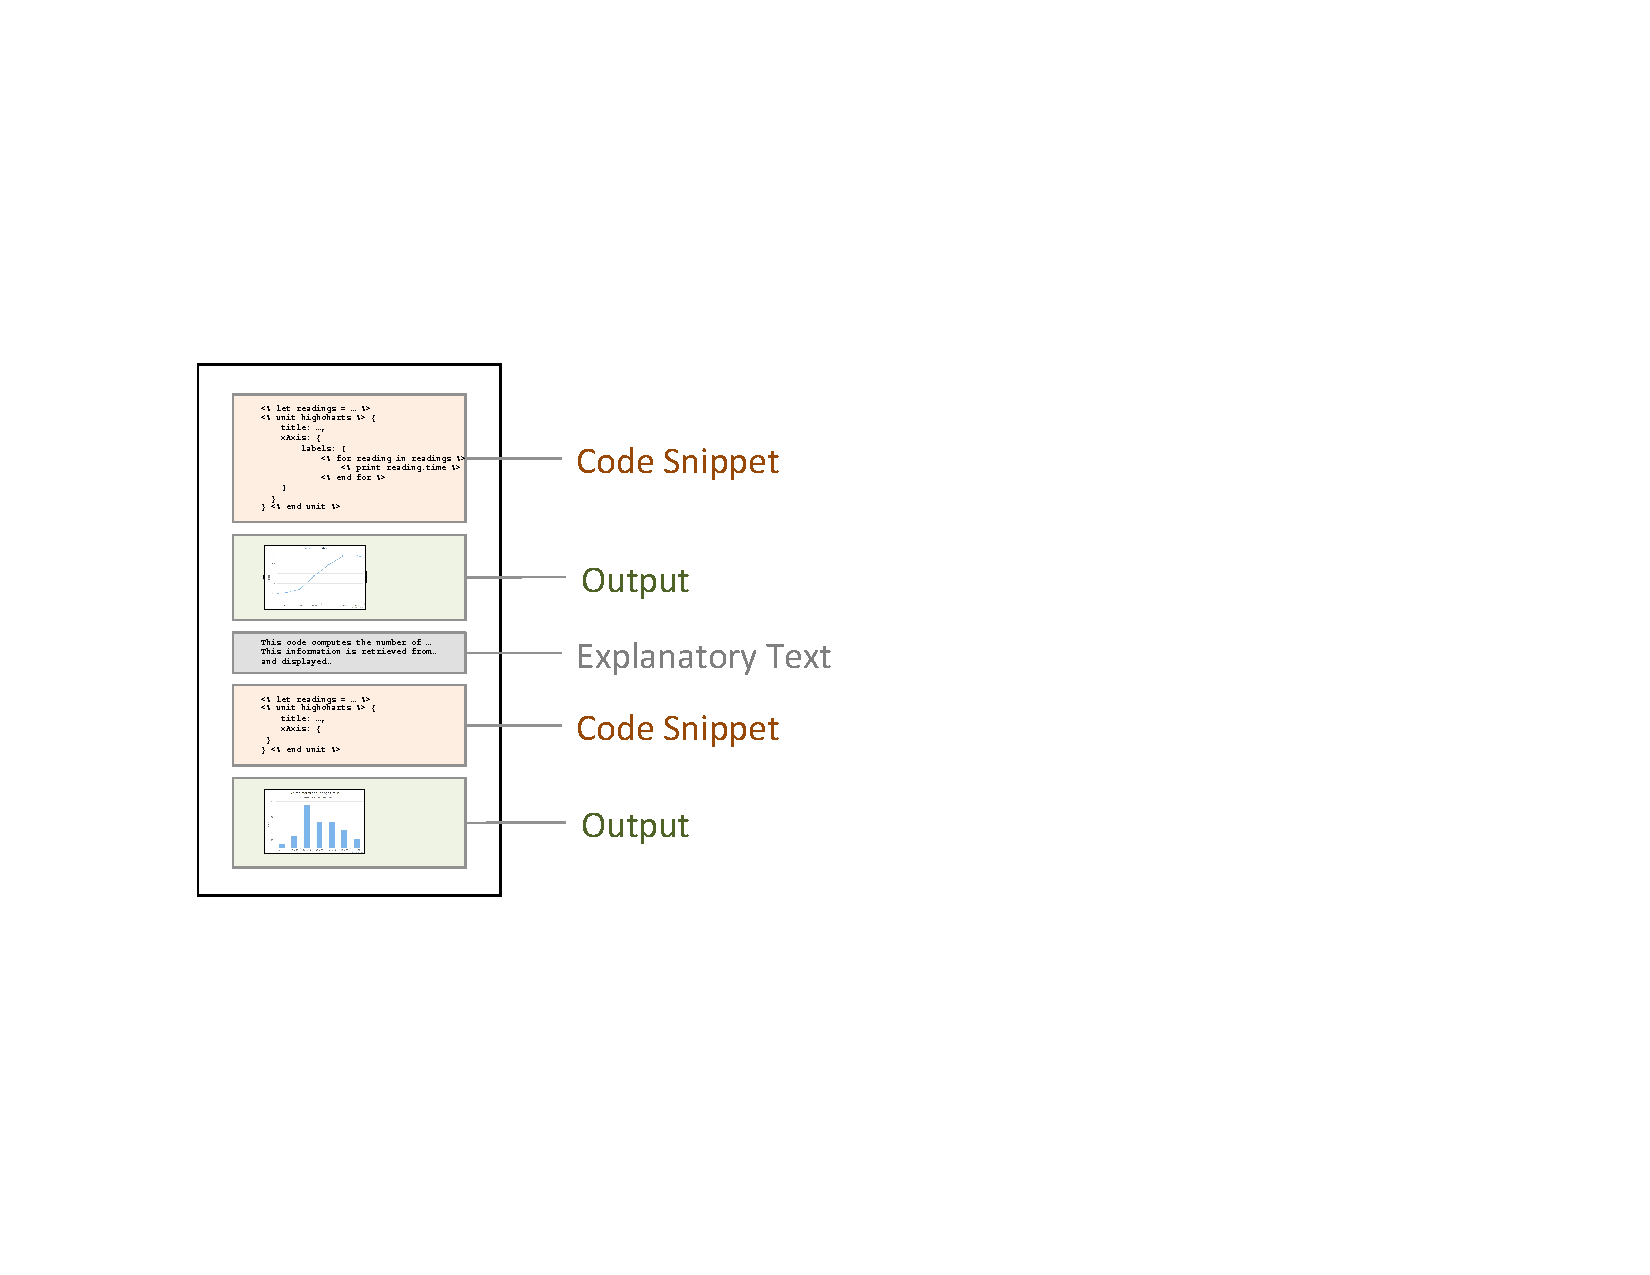
\includegraphics[width=0.7\columnwidth]{figures/notebook2.pdf}
	\caption{Notebook interface}
	%\vspace{-15pt}
	\label{figure:notebook-interface}
\end{figure}

\eat{
However, interactive notebooks are still suboptimal with regard to ease of use and productivity for data analysts. 
Retrieving, processing and visualizing data requires technical expertise that often exceeds the skill-set of a typical data analyst. Specifically, such steps require data transfers and package installations on the notebook server, in order to be used in an analysis. Such tasks fit the job description of a system administrator rather than a data analyst. \costas{downplay the sysadmin aspects of it.} Additionally, even after the environment has been setup, the data analyst has to read long documentation files that explain how to programmatically interact with such tools and she often has to spend significant effort writing plumbing code in order combine their functionality.
}


\eat{
However, interactive notebooks are still suboptimal with regard to ease of use and productivity for data analysts. Retrieving, processing and visualizing data involves reading lengthy documentation pages that describe each library's API and writing complex imperative plumbing code that combines their functionality. Both these steps, are not only very time consuming but also require technical expertise that exceeds the skill-set of a typical data analyst. 
\costas{If I understand the new instructions this last paragraph should be removed, correct?}
}

\eat{
Besides the aforementioned limitations that impact data analysts, notebooks also have limitations that impact the, potentially non-technical, readers of the published notebooks. Particularly, while notebooks can contain visualizations that showcase important aspects of a data analysis, the readers cannot interact with the provided visualizations in the same way they could if these visualizations were part of a typical OLAP dashboard application. Specifically, even if the analyst that composed the notebook used third-party web-based visualization libraries that support user interaction, this interaction can only cause local changes to the visualization \cite{Bokeh, plotly, ipyvega, Altair} the reader interacts with and cannot trigger additional data retrieval, computation or mutations to other visualizations that are included in the notebook. For this reason, only code-literate readers, capable of extending the notebook with more coding snippets, are able to further explore the underlying data (or examine additional hypotheses about the underlying data), while the rest are limited to passively reading the generated notebook.
}


Jupyter notebooks, however, have limitations that impact the exploratory capabilities that can be performed by the potentially non-technical, readers of the published notebooks. Particularly, while notebooks can contain visualizations that showcase important aspects of a data analysis, the readers cannot interact with them in the same way they could if these visualizations were part of a typical OLAP dashboard application. Specifically, even if the analyst that composes the notebook uses third-party web-based visualization libraries \cite{Bokeh, plotly, ipyvega, Altair} that support user interaction, the default side-effect of this interaction is to only cause local changes to the visualization the reader interacts with and, therefore, do not trigger additional data retrieval, computation or mutations to other visualizations that are included in the notebook (which could be generated by subsequent coding blocks). Adding more elaborate side-effects that can perform such tasks requires complex event-driven logic that is typically used by web developers (in MVC applications) which entails a more advanced skill-set that data analysts might lack. For this reason, only code-literate readers, capable of extending the notebook with more coding snippets, are able to further explore the underlying data (or examine additional hypotheses about that data), while the rest are limited to passively reading the generated notebook. 


We are investigating two methods, that can be used for the creation of reactive notebooks. Both these methods describe side-effects implicitly using a view-over-data approach, without requiring additional event-driven logic. The first method, presented in this paper, is using FORWARD  \cite{SIGMOD2010,CIDR2011} and its DSL, with two differences: (a) Unlike FORWARD where the presentation layout is determined by markup \cite{forward_online}, \projname\ assumes that the FORWARD DSL script is a sequence of pairs consisting of computation (essentially, computing a view) and a visual unit that visualizes the view, (b) the second difference is the extension of FORWARD towards interfacing with Python code - in particular, with Python functions. The second approach is based on using existing Jupyter (Python) coding blocks, (which describe the initial visualizations) and inferring how the outcome of each statement would be affected given a mutation. In this paper we will describe the first approach as the DSL makes static analysis and change propagation, needed for efficiency, far easier.

\eat{

In order to add such OLAP-like functionality to notebooks, a data analyst has to explicitly implement event-driven logic for every UI event that might occur. This process however is not trivial, manually specifying elaborate side-effects for each event that might occur is an extremely arduous and error-prone task, especially, when multiple events cause mutations to the same visualizations of the notebook. This coding style is used by web developers (in MVC frameworks) when building fully-fledged applications, and it typically requires advanced skill-set that data analysts might lack. At the same time, such event-driven programming style is not typically used in Jupyter notebooks. Lastly, note that the provided logic executed after each event may need to mutate visualizations generated by subsequent coding blocks, this functionality however, is not supported by most third-party visualization libraries.

}


\costas{Does this point belong to both the reader and the data analyst of the notebook? Regardless of the technical expertise of the analyst, building a reactive dashboard just cannot be done in a notebook that contains multiple cells.}


\costas{reviewer 1: Interactive visualizations are indeed supported in Jupyter via JS libraries -- e.g. Reactive Vega, Altair, Plotly, PivotTable, etc. You say it's not possible, and in the next paragraph you say it *is* possible BUT only with local changes.}

\costas{Is there a problem with my writing here? We should make it clear that we meant that it doesn't work across visualizations/data access/computations described across multiple cells}

\costas{reviewer 1: b. But that is incorrect also! ipywidgets allow reactivity, so that interactive visualizations can trigger data retrieval, computation and data mutation. If you pass (say) Python state into the widget, it can use that state to trigger Python calls to data backends.Now perhaps that hasn't been wrapped up neatly yet with a viz library into a DSL (I'm not sure), but it's definitely quite possible.}

\costas{The problem is that the data obtained from the backend cannot be consumed by visualizations that exist in subsequent coding blocks. The interesting sequence that cannot be currently performed in notebooks is: Going from (1) user interaction within charts to (2 - optional) data access to (3 - optional) data processing to (4) (ideally incremental) reevaluation of subsequent charts/graphs. In ViDeTTe each of these steps could appear in separate notebook cells.
One could implement what the reviewer suggests in a single cell (although not a lot of visualizations can be visible in the limited space where the output of a single cell appears) but that's not how analysts use notebooks, this is how a web developer would build an application that countains visualizations}


\costas{Reviewer 2: The "reader`` in this case is acting the role of "interactor`` They are doing more than simply reading the notebook, but rather interacting with it. One wonders if there might be different goals for true notebook readers. }

\costas{We should address this (perhaps we should add the "freeze" feature mentioned in my email?) 2/3 reviewers touched on this subject.}

\noindent {\bf Contributions.}
In order to offer the capability to describe reactive behavior without requiring explicit event-driven logic in notebooks, we extend Jupyter with the  {\projname} notebook engine. The main contributions of this extension are: (a) visual constructs, capable of collecting the reader's input as they interact with the produced visualizations, (b) A declarative template language that can be used to declaratively describe computation, data transformations and user input collection, (c) An algorithm, capable of propagating changes between co-dependent visual constructs and computations, which introduces a truly reactive behavior to notebooks. These reactive capabilities, enable non-technical readers to further explore the underlying data used in an analysis.

\costas{I think it's fair to say that the first author was against the first contribution (because there are existing libraries that perform these individual tasks, which I also mentioned in the next sections). Should this be removed? I think we have a great way of combining the functionality provided by these modules in a declarative way which is superior to the way someone would interface these individual libraries (especially when dealing with event-drive reactivity) but this is expressed by the second contribution. What do you think?}

\eat{
\begin{compact_enum} 
\item visual and data retrieval constructs, that simplify the process of data retrieval and visualization, for data analysts, 
\item A declarative template language that can be used for describing computation, data transformations and user input collection, \eat{\yannis{shouldn't this item be bigger? It's not just input collection: doesn't it also define control flow?}}
\item A propagation algorithm, that utilizes visual and data retrieval constructs, combined with templates in order to introduce a reactive behavior to notebooks. These reactive capabilities, enable non-technical readers to further explore data, without requiring any coding skills. 
\end{compact_enum}
}
\eat{
The remainder of this paper is organized as follows: Section ?? discusses the architecture of the {\projname} framework. Due to space limitation, we focus on those aspects that can be useful as a notebook extension. Section ?? presents our example data analysis. Finally, Section ?? concludes the paper.
}

\eat{
\noindent {\bf Contributions.}
To sum up, we extend interactive notebooks with the  {\projname} notebook engine. The main contributions of this extension are: (a) visual and data retrieval constructs, that simplify the process of data retrieval and visualization, (b) A declarative template language that can be used for specifying computation, data transformations and user input collection, (c) A propagation algorithm, that utilizes visual and data retrieval constructs, in association with a template language in order to introduce a reactive in notebooks. 
}
\eat{

\begin{itemize}
	\item \textit{Expressive template language:} Prior work, treats a page as a database view. Building on that, our template language goes beyond SQL query and view definition in both style and fundamental expressiveness. It is a mixture of query as well as web templating language that works on ordered (arrays) and semi-ordered (JSON) data. 
	\item \textit{Easy data retrieval:} Our framework supports communication with all major database types, such as Postgress, MongoDB, SQL etc, eliminating the need for individual DB drivers. Furthermore, using {\projname}, user access credentials for the database server(s) are stored in a configuration file, eliminating the embarassingly insecure practice of typing usernames and passwords in notebook cells vidible to everyone.
	\item \textit{Inline JSON operations:} The primary data structure used in {\projname} is JSON arrays. {\projname} combines the intuitive nature of JSON with the ability to write inline JSON operations, resulting in a clean, structured and readable code.
	\item \textit{Variable binding:} Analysts can easily ``bind'' variables using our template language. ``Binding'', results in automatic re-execution of notebook cells that contain those variables upon a change. {\projname} will trigger execution of the appropriate cells without any extra coding effort. As we show later, combined with inline JSON operations, binding becomes an incredibly versatile tool.

%	\item \textit{Declarative semantics:} {\projname} implements formal declarative \textit{Model-View-View-Model} (MVVM) semantics. \remark{Fill in why this is a good thing. I have no idea.}
%	\item \textit{Expressive template language:} Prior database work, treats a page as a database view. Building on that, our template language goes beyond SQL query and view definition in both style and fundamental expressiveness. It is a mixture of query as well as web templating language that works on ordered (arrays) and semi-ordered (JSON) data. 
%	\item We allow in-line declarative code directly in JSON...
\end{itemize}

}


\eat{
\begin{figure*}
	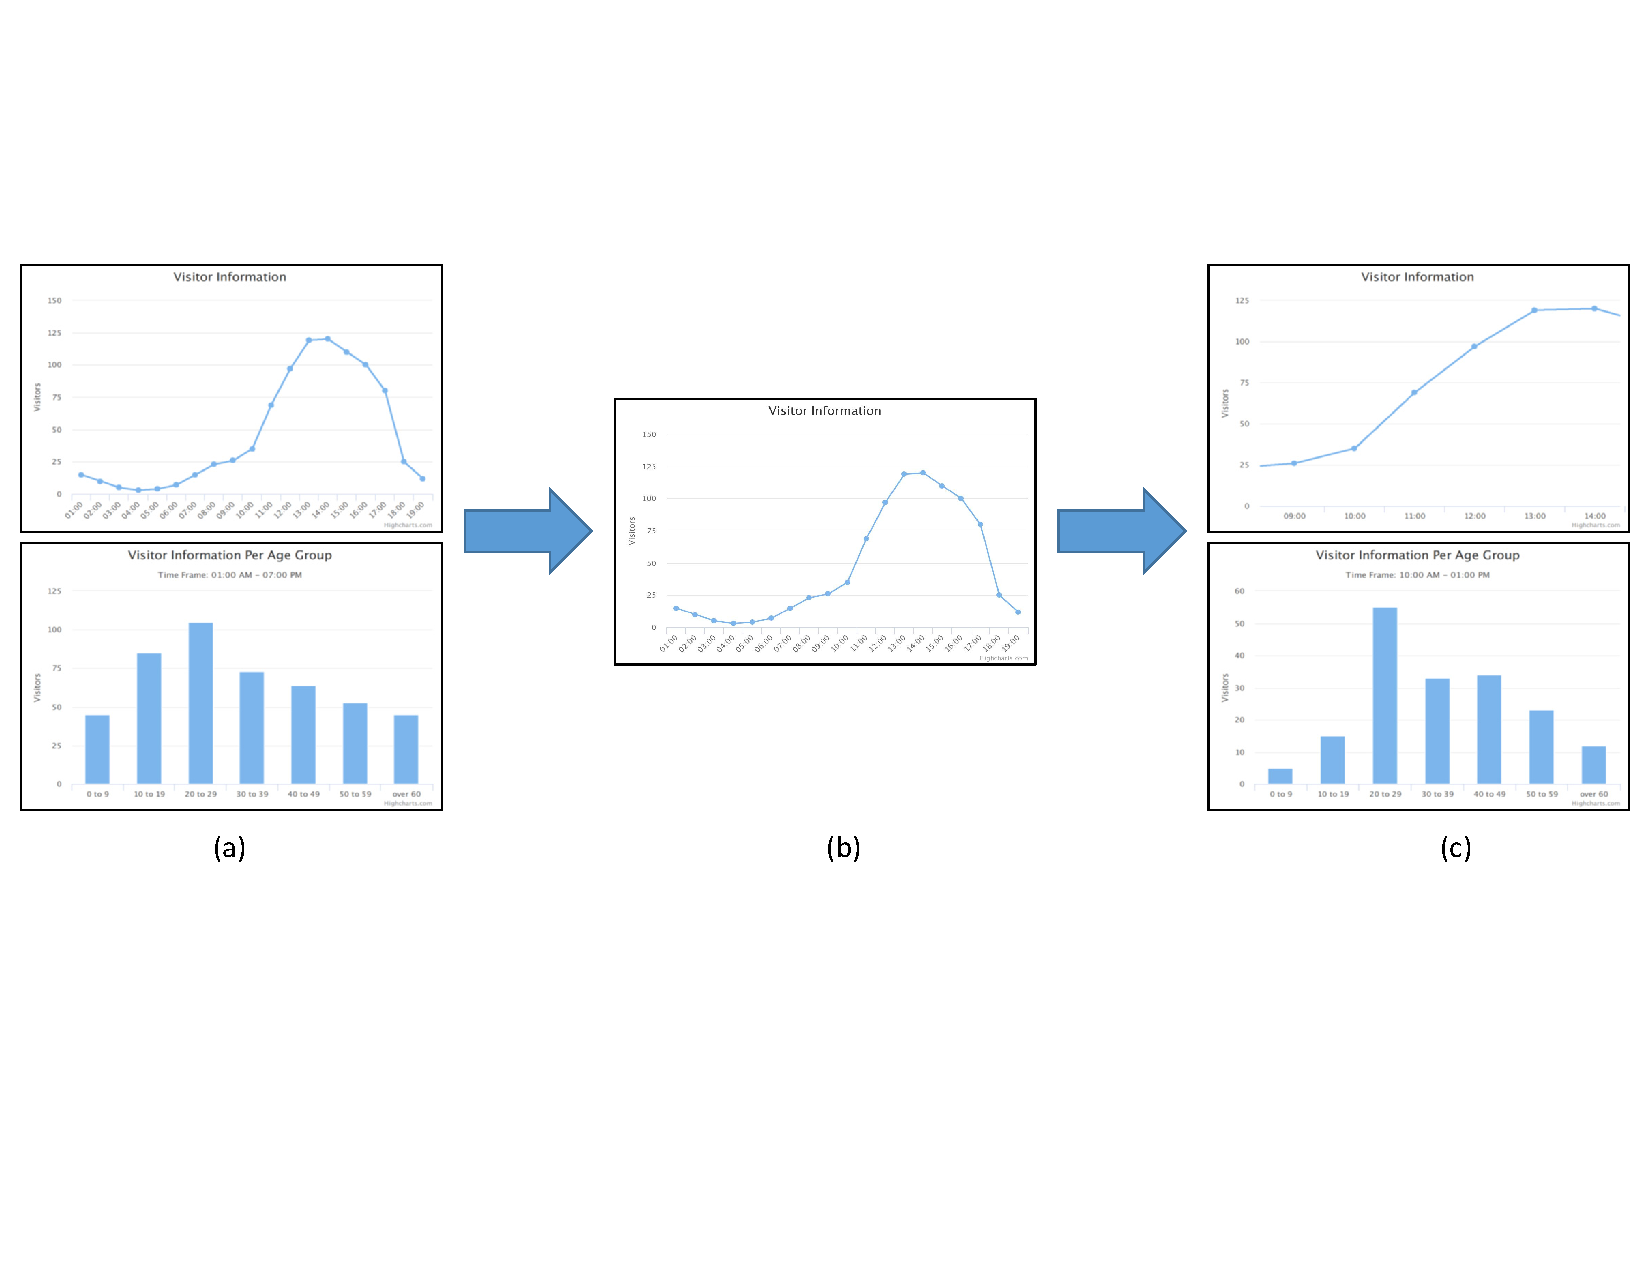
\includegraphics[width=\textwidth]{figures/highchart_final_a.pdf}
	\caption{Demonstration of interactive charts. The analyst's selection automatically updates the second plot (right).}
	\label{fig:vision}
\end{figure*}
}
\eat{
\begin{figure*}
	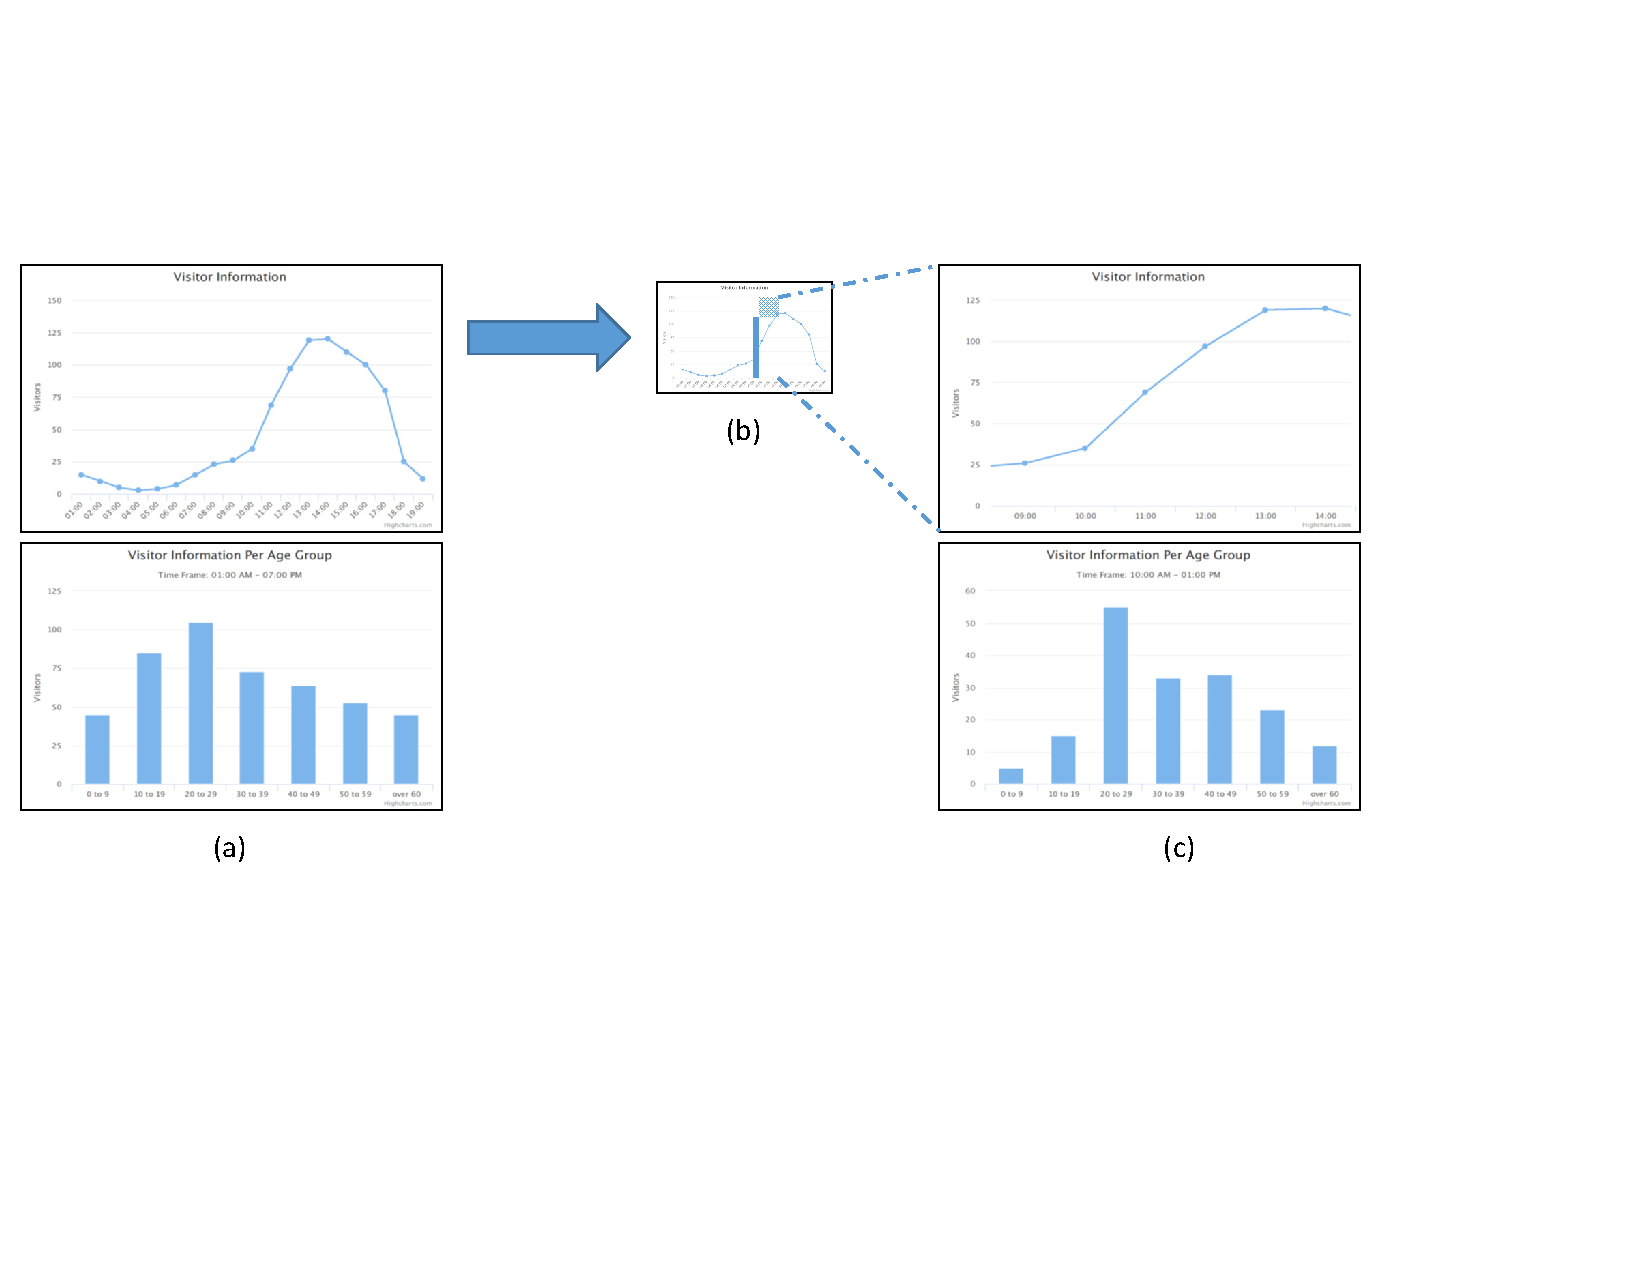
\includegraphics[width=\textwidth]{figures/highchart_final_b.pdf}
	\caption{Demonstration of interactive charts. The analyst's selection automatically updates the second plot (right).}
	\label{fig:vision}
\end{figure*}
}
\eat{
\remark{Ok I thought about it and I propose the following modifications in the paper structure (Nothing major - just moving text around to make it more readable): We begin with a good discussion about the vidette features that can help notebooks in section 2. We then show the entire walkthrough in one section (Section 3). By now, the reader knows what vidette can do so it will be easier to follow and understand the code we show.}
}
 \eat{
We address these issues, by extending interactive notebooks with the  {\projname} framework. {\projname} notebooks support a new template language capable of facilitating common data analysis tasks. The main contributions of this extension are:

\begin{itemize}
	\item \textit{Expressive template language:} Prior work, treats a page as a database view. Building on that, our template language goes beyond SQL query and view definition in both style and fundamental expressiveness. It is a mixture of query as well as web templating language that works on ordered (arrays) and semi-ordered (JSON) data. 
	\item \textit{Easy data retrieval:} Our framework supports communication with all major database types, such as Postgress, MongoDB, SQL etc, eliminating the need for individual DB drivers. Furthermore, using {\projname}, user access credentials for the database server(s) are stored in a configuration file, eliminating the embarassingly insecure practice of typing usernames and passwords in notebook cells vidible to everyone.
	\item \textit{Inline JSON operations:} The primary data structure used in {\projname} is JSON arrays. {\projname} combines the intuitive nature of JSON with the ability to write inline JSON operations, resulting in a clean, structured and readable code.
	\item \textit{Variable binding:} Analysts can easily ``bind'' variables using our template language. ``Binding'', results in automatic re-execution of notebook cells that contain those variables upon a change. {\projname} will trigger execution of the appropriate cells without any extra coding effort. As we show later, combined with inline JSON operations, binding becomes an incredibly versatile tool.

%	\item \textit{Declarative semantics:} {\projname} implements formal declarative \textit{Model-View-View-Model} (MVVM) semantics. \remark{Fill in why this is a good thing. I have no idea.}
%	\item \textit{Expressive template language:} Prior database work, treats a page as a database view. Building on that, our template language goes beyond SQL query and view definition in both style and fundamental expressiveness. It is a mixture of query as well as web templating language that works on ordered (arrays) and semi-ordered (JSON) data. 
%	\item We allow in-line declarative code directly in JSON...
\end{itemize}
}


%In this paper, we demonstrate the use of {\projname} via a walkthrough example. Specifically, we want to use website access data to plot an access count over time histogram. We also want to plot the recorded user demographics (with focus on age groups). We then want to have the ability to interact with the histogram plot and select a time region. This action should automatically update the second plot with the user demographics in the selected time window. 
%
%Without loss of generality, we assume a Jupyter server, where the analysts develop their notebooks and a different database server where data is stored. To retrieve the entirety of the required data, we have to query two different databases and join the returned JSON files. Figure ?? shows how our databases are organized. Our fictional analyst will perform the following high-level tasks:
%
%\begin{itemize}
%	\item Data retrieval from remote databases. 
%	\item Data curation: Join data and prepare for visualization.
%	\item Data visualization.
%\end{itemize}
%
%The remainder of this paper is organized as follows: Sections \ref{section:dataretrieval} -- \ref{section:visualization} present a direct comparison of using {\projname} and an imperative language such as Python in order to complete the tasks of our example. Throughout these sections, we demonstrate some of the main contributions of {\projname}. Section \ref{section:discussion} provides further discussion regarding our proposed extension and presents other useful aspects of it not used in our walkthrough. Finally, Section \ref{section:conclusion} concludes the paper.


\section{Running Example}


\begin{figure}[t]
  \centering
  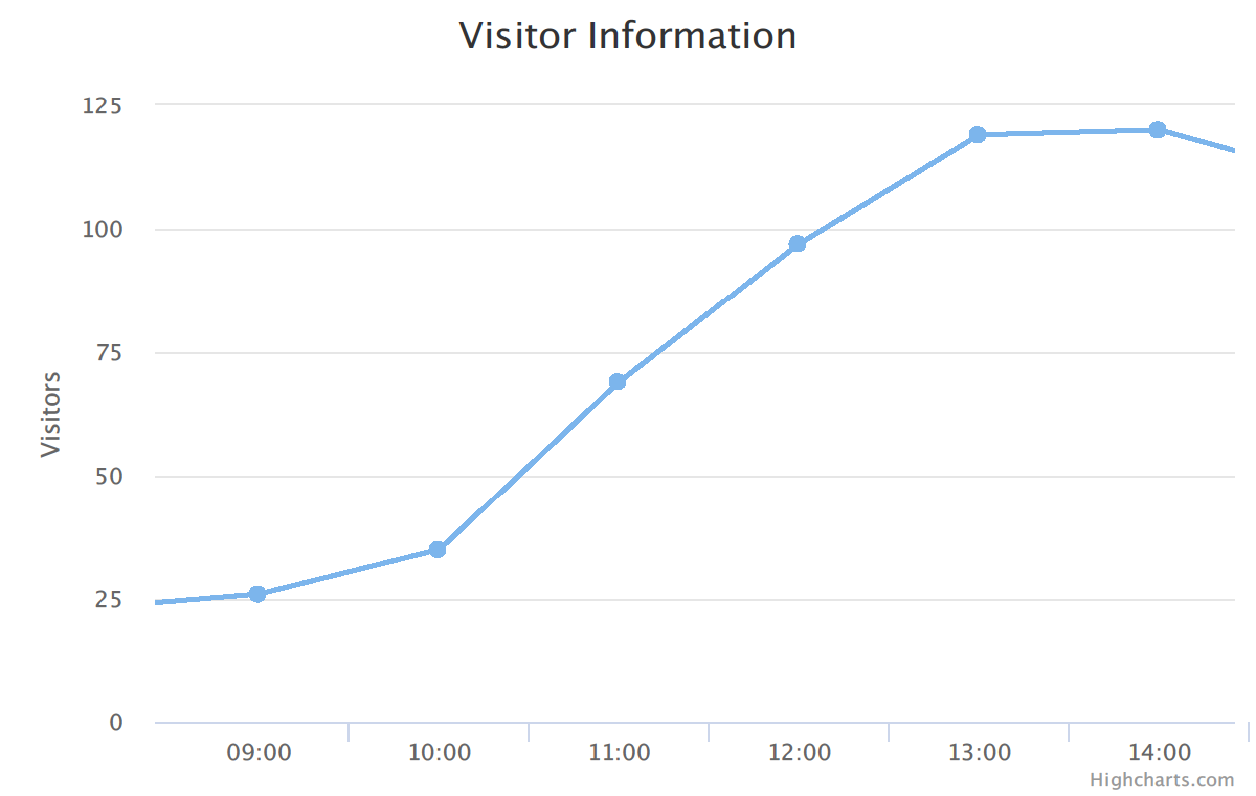
\includegraphics[width=0.8\columnwidth]{figures/first-line.png}
  \caption{Line chart showing visitors per hour}
\label{figure:first-running-example:first-line-chart}
  %\vspace*{\floatsep}% http://tex.stackexchange.com/q/26521/5764
   %\vspace*{0.1cm}
  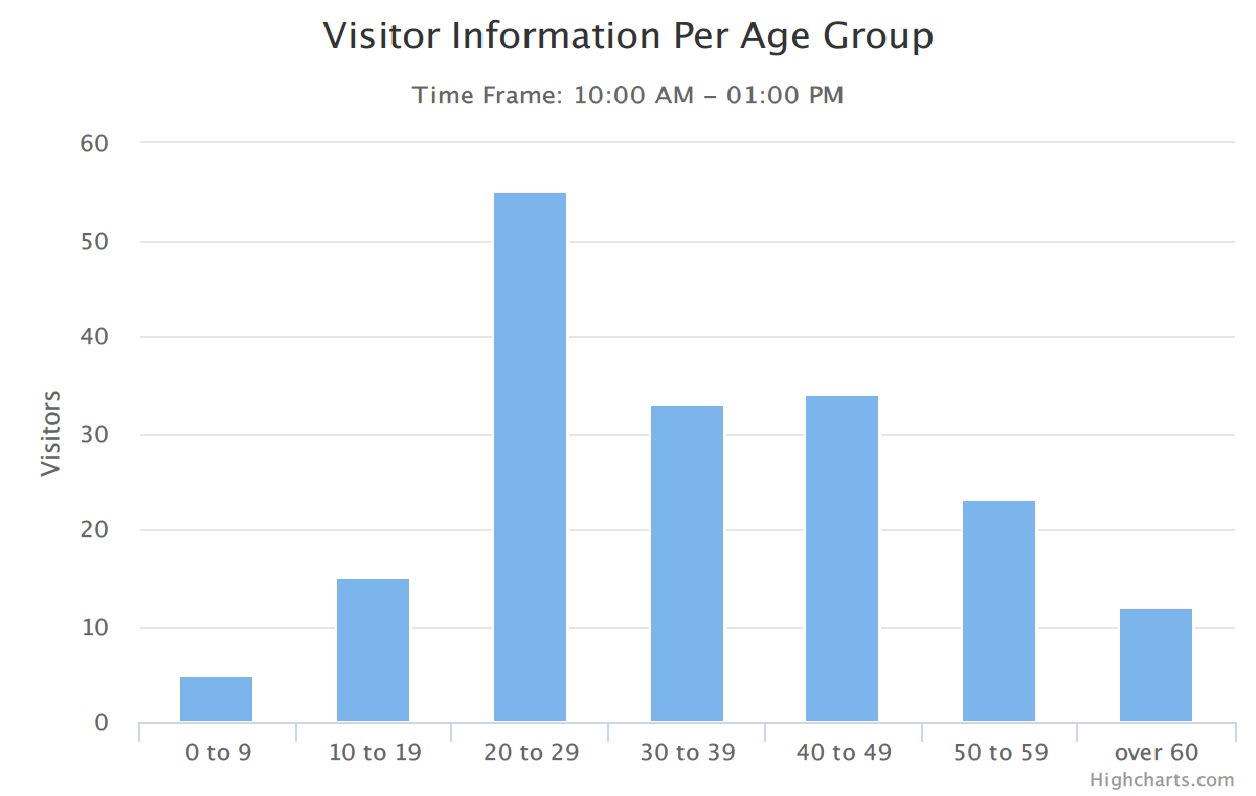
\includegraphics[width=0.8\columnwidth]{figures/first-bar.png}
  \caption{Bar chart showing age groups of visitors}
  \vspace{-15pt}
  \label{figure:first-running-example:first-bar-chart}
  
\end{figure}

\begin{table}
\begin{center}

\begin{tabular}{|c|c|c|c|c|c|}
\hline 
\multicolumn{6}{|c|}{Page Views} \\ 
\hline 
id & vid & url & time & date & revenue \\ 
\hline 
\end{tabular} 

\hfill

\begin{tabular}{|c|c|c|c|c|c|}
\hline 
\multicolumn{6}{|c|}{Visitors} \\ 
\hline 
vid & name & lastname & username & age & gender \\ 
\hline 
\end{tabular} 

\end{center}
\caption{Schema description of database tables.}
\vspace*{-30pt}
\label{tab:schema}

\end{table}


In order to illustrate the issues with existing notebooks and describe the extensions in \projname\, we will use the following example of a potential analysis:

\begin{example}
	
\eat{	
	
Consider a data analyst, working for a news portal website. The analyst wishes to create a notebook that extracts and presents information about the demographics of the website's reader-base during particular hours. More specifically, the analyst wants to construct a chart showing the number of readers that visit the website during the day; then based on this information, she would like to extract the age groups of the visitors, during various hours of that day and present the results to the portal editor. Figure \ref{figure:first-running-example:first-line-chart} shows the graph that displays the number of visitors per hour in a line chart and Figure \ref{figure:first-running-example:first-bar-chart} displays the age groups of the visitors in a bar chart. By doing this, the analyst can convince the portal editor to publish more articles and advertisements that target particular age groups during hours in which they visit the portal the most, thus maximizing the portal's revenue and reader's satisfaction.
}

\eat{
Consider a data analyst, working for a news portal. The analyst wishes to convince the lead editor of the portal that by publishing more articles and advertisements that pertain to particular audiences during specific time-windows of the day, they can maximize the portal's revenue. In order to achieve this, the analyst intends to obtain data that contain the number of readers that visit the website during the day; then for various time-windows she would like to obtain and plot the demographics of the portal's visitors (for instance, the visitors' age groups) during these hours and lastly compute and plot the portal's actual and the predicted revenue. 
}

Consider a data analyst, working for a news portal. The analyst wishes to convince the lead editor of the portal that by publishing more articles and advertisements that pertain to particular audiences during specific time-windows of the day, they can maximize the portal's revenue. In order to achieve this, the analyst intends to obtain and plot the number of readers that visit the website during the day; then for various time-windows she would like to obtain information about the readers' demographics (for instance, the visitors' age groups) and plot the result. Lastly, she would like to compute the portal's actual and predicted revenue (using a linear regression model) and plot the the results, side-by-side, thus illustrating whether there is room for improving revenue. 
\end{example}

Note that, in this example, we can identify two types of users, the code-literate data scientist and the non-technical editor of the portal.

\eat{
\begin{figure}[ht]
  \centering
  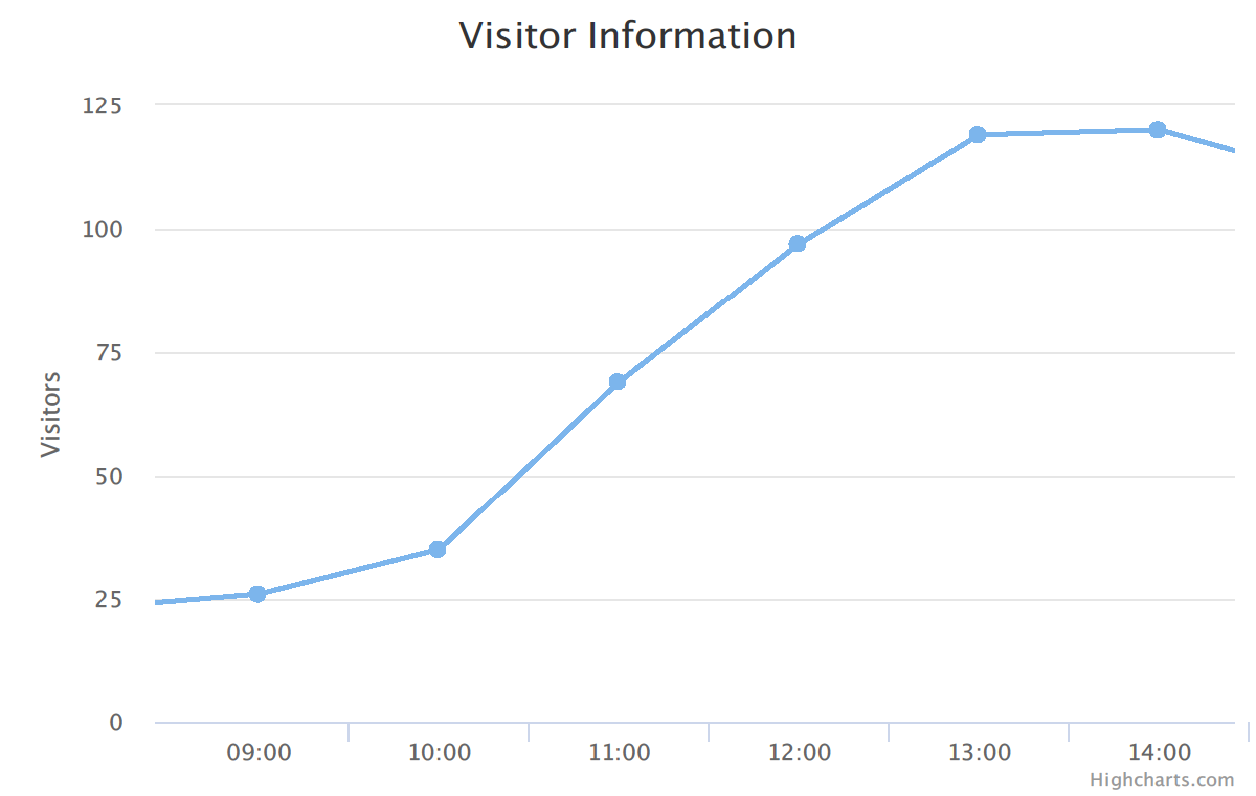
\includegraphics[width=0.8\columnwidth]{figures/first-line.png}
  \caption{Line chart showing visitors per hour}
\label{figure:first-running-example:first-line-chart}
  %\vspace*{\floatsep}% http://tex.stackexchange.com/q/26521/5764
   %\vspace*{0.1cm}
  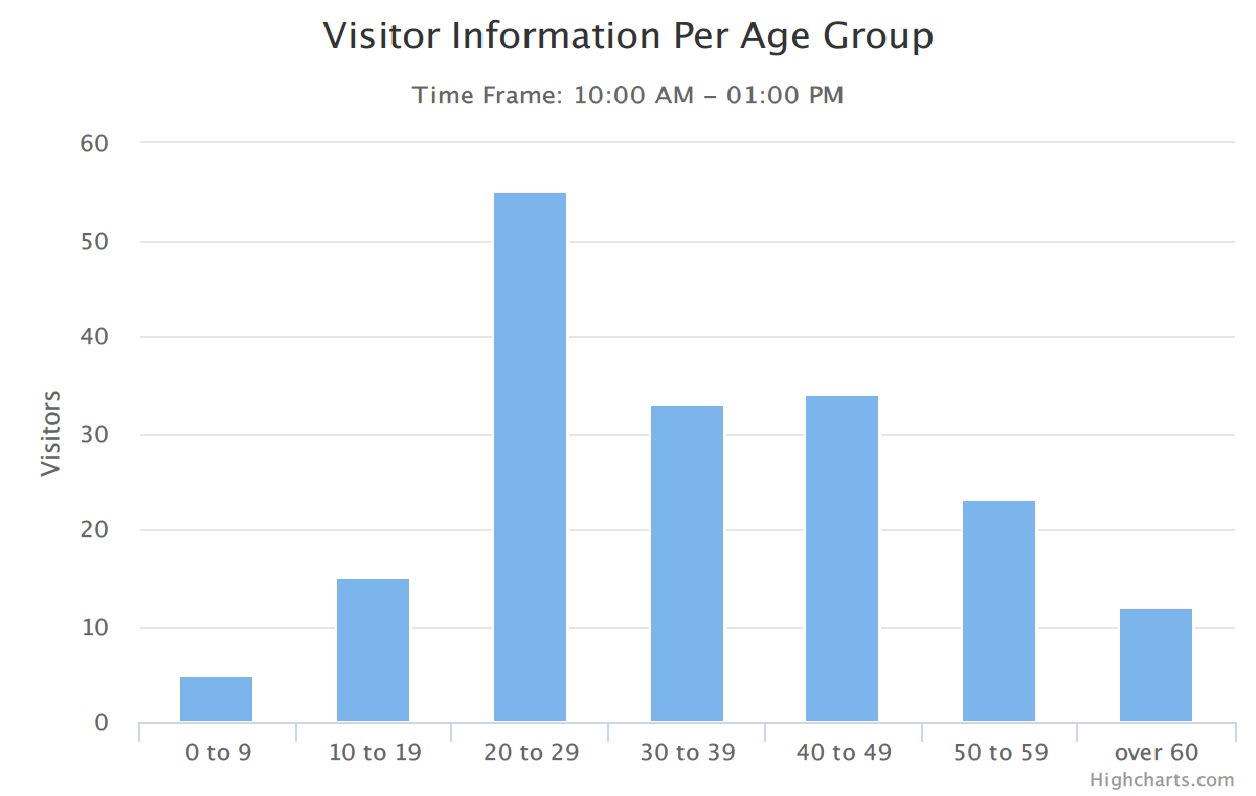
\includegraphics[width=0.8\columnwidth]{figures/first-bar.png}
  \caption{Bar chart showing age groups of visitors}
  \label{figure:first-running-example:first-bar-chart}
\end{figure}
}



\costas{Should section 2 be changed in any way?}






%\vspace*{-0.4cm}
\section{Data Analysis using Jupyter}


\begin{figure*}[hbt!]
\centering
	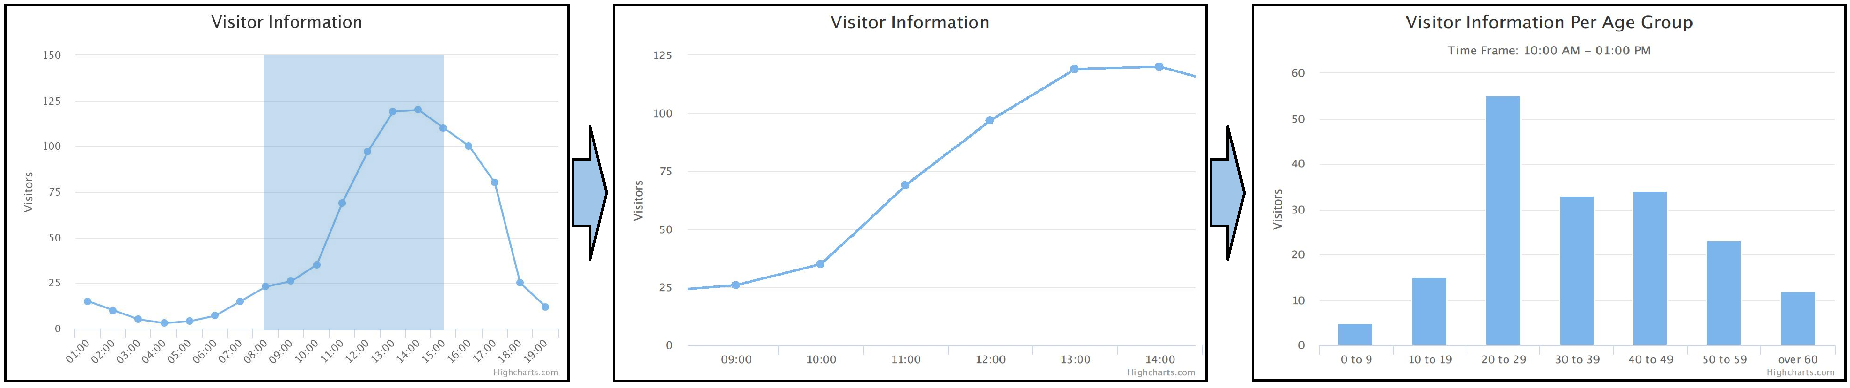
\includegraphics[width=1\textwidth]{figures/reactive-processing2.pdf}
	\caption{Demonstration of reactive charts. The reader's selection automatically updates both charts.}
	\label{fig:reactive-data-processing}
	\vspace{-6pt}
\end{figure*}



\costas{reviewer 1: c. Logging into databases, etc using Python libraries is not really harder today than what you show in the paper. See the ipython-sql library and its use of SQLAlchemy. For us database folks, this is already a standard way to work with Python and notebooks. d. You seem to indicate that there is an unsolved object-relational data type conversion problem in Python/SQL. But Pandas dataframes do a fine job with this, even over something like ipython-sql. This is a non-issue for Python notebook users today. }

\costas{ipython-sql is a python magic command that let's you inline queries in Jupyter and it returns the result in a pandas dataframe. This tool lacks the interactive aspect which is required in order to build a reactive analysis. You cannot issue a parameterized query that is executed every time the user interacts with a visualization (I verified this).}


We will now describe how a data scientist would perform this analysis with a traditional interactive notebook and illustrate how the limited interactive capabilities affect the level of data exploration that can be performed. We assume that the news portal maintains data about its reader-base in a Postgres database. Table \ref{tab:schema} shows a potential schema, that could be used for storing visitor information. The database contains two tables, namely ``Page Views" and ``Visitors"; table ``Visitors" contains information about each reader, such as the reader id, name, lastname, username, age and gender. The table ``Page Views" maintains a tuple for each visit, and it consists of a visit id, the visitor id (foreign key referencing the visitor), the url of the visited page, the hour and date in which the user visited the website and the revenue collected during this visit. The reader information could have been retrieved, with their permission, from various social media services (such as Facebook, Google etc). 

\noindent {\bf Data analysis steps.}
In order to construct this notebook, the data analyst must (a) retrieve  website access information from the database, by joining the two tables on the visitor id (b) generate a plot that shows the number of users that visit the website during the day, (c) issue a query that counts the number of visitors per age group for a meaningful set of hours (time frame), (d) create a bar chart that shows the number of visitors per age group, (e) use an already trained predictive model in order to predict the expected revenue for the selected time window and (f) plot a bar chart, showing the actual and the predicted revenue generated in selected time window. Note that in order to perform these steps, the data analyst must employ a plethora of third-party Python libraries (database drivers, machine learning and visualization libraries etc.,) used for data access, data processing and visualization. Each of those libraries expects or returns data in a predefined schema, therefore, the analyst must manually perform schema transformations for each library they want to use. Most importantly, note that selecting a meaningful time frame (step c) in this analysis, is of utmost significance, because it will affect all the remaining steps of this analysis, and ultimately the insight, the portal editor will gain, about potential ways to increase the revenue

 \eat{
In order to retrieve website access information from the database, the data analyst, needs to employ third-party Python drivers. After establishing the connection with the database system, and issuing the queries, the analyst, is able to consume the results using the internal, to the library, data types. Afterwards, the analyst needs to perform (schema) conversions in order to invoke the respective visualization library, with the appropriate arguments, thus constructing the first visualization.
}

\costas{Repeating comment here: d. You seem to indicate that there is an unsolved object-relational data type conversion problem in Python/SQL. But Pandas dataframes do a fine job with this, even over something like ipython-sql. This is a non-issue for Python notebook users today. Separate comment: It felt to me that you are unfamiliar with Jupyter Lab, Pandas, and the rest of the standard toolchain that people use. Maybe that's not true! But it comes across that way. For example, it's odd that you return dictionaries rather than dataframes, and your comments on "Data conversion" reinforces that feeling. If you do know your stuff, then for some reason you are not integrating with the community's favorite libraries. If that's the case, you might be more thoughtful in explaining why your counter-cultural approach is good.}

\costas{The point I was trying to make here is that regardless of whether we integrate with dictionaries or dataframes, the analyst still has to read the documentation page of the visualization library and manually convert the data into the format/schema that is expected by the visualization library. Dataframes are indeed used a lot by many libraries however they cannot capture nested data while dictionaries can. Additionally, dictionaries are natively supported by Python while Pandas is an external library. Also while some tools interface well with pandas many of them actually require conversions into python dictionaries/arrays (here is an example using plotly that requires a dataframe to be converted into a dictionary: https://plot.ly/ipython-notebooks/cufflinks/, plotly has the same issue) as shown in the same link because of this missmatch, additional libraries have to be used to simplify this data conversion (i.e., cufflinks). On the other hand all libraries interface with python natively supported types (i.e., dictionaries) additionally dataframes can be converted into (flat) dictionaries with one command (and the other way around)... If he considers integration with dataframes (which again are simply flat dictionaries) so critical, we can support that as well. On a separate note, Jupyter Labs is simply a more advanced web IDE for creating ipython notebooks. I don't understand how that's comparable to vidette (one can use Jupyter labs to build a jupyter notebook that employs vidette...)}

\eat{
The next step is for the analyst to issue a query that counts the visitors per age group for a set of selected hours and construct a bar chart showing the result. The obtained dataset will also go through a machine learning package (for instance, the scikit-learn package \cite{scikit-learn}), that employs a linear regression model to predict the expected revenue during the selected hours. The predicted revenue will be plotted in a new graph next to the actual revenue produced during these hours. Note that selecting a meaningful time frame, is of utmost importance, because it will affect all the remaining steps of this analysis, and ultimately the insight, the portal editor will gain, about potential ways to increase the revenue. 
}




 % Template and template instance figures
 \begin{figure*}[hbt!]
 \centering
 %
 %
 \begin{minipage}[c]{7cm}
 %
 \begin{minipage}[c]{7cm}
 \begin{code}
 \textbf{<\% let} readings = sql(
    SELECT count(time) as visits, time
    FROM (SELECT * FROM page_views pv 
   	     join visitors v 
          on pv.v_id = v.vid) AS joined_table
    GROUP BY time ORDER BY time ASC \textbf{\%>};)
 \end{code}
 \vspace*{-0.2cm}
 \subcaption{Data retrieval}
 \label{figure:first-running-example:data-retrieval}
 \vspace*{0cm}
 \end{minipage}
 
 
 \begin{minipage}[c]{7cm}
 	\begin{code}
 \directive{unit}{highcharts} \{
   title: 'Visitor information' , type: 'line',
   xAxis : \{ 
     labels : ['08:00','09:00'...], min : '08:00', max : '22:00'
   \}
   series: [\{ data: [ \{y:15\}, \{y:10\}...] \}]
 \} \directive{end unit}{}
 	\end{code}
 	\vspace*{-0.2cm}
 	\subcaption{Unit with evaluated unit state}
 	\vspace*{0cm}
 	\label{figure:running-example:unit-body}
 \end{minipage}
 \begin{minipage}[c]{7cm}
 	\begin{code}
 readings = [ \{visits: 15, time: '08:00'\},...]
 	\end{code}
 	\vspace*{-0.2cm}
 	\subcaption{Query Result}
 	\label{figure:running-example:query-result}
 	\vspace*{0cm}
 \end{minipage}
 %
 \vspace*{0cm}
 \end{minipage}
 \hspace{2cm}
 \begin{minipage}[c]{6cm}
 
 \begin{minipage}[c]{7.5cm}
 \begin{code}
   \directive{init}{min_time = '01:00'} 
   \directive{init}{max_time = '24:00"} 
   \directive{unit}{highcharts} \{
     title: 'Visitor information',
     type: 'line',
     xAxis : \{ 
       labels : [
         \directive{for}{reading \textbf{in} readings} 
           \directive{print}{reading.time} 
         \directive{end for}{}],
       min : \directive{bind}{min_time},
       max : \directive{bind}{max_time}
     \}
     series: [\{
       data: [ \directive{for}{reading \textbf{in} readings}
           \{
             y  : \directive{print}{reading.count}
           \}  
           \directive{end for}{} ]
     \}] \} \directive{end unit}{}
 \end{code}
 \vspace*{-0.2cm}
 \subcaption{Template generating unit state of first chart}
 \vspace*{0cm}
 \label{figure:first-running-example:main-template}
 \end{minipage}
 \end{minipage}
 \vspace*{-0.3cm}
 \caption{Declarative data retrieval, evaluated unit state and Template describing unit state for running example}
 \vspace*{-0.3cm}
 \end{figure*}
 
 \noindent {\bf Limited interactivity impacts exploratory capabilities.} Unfortunately, there is no straightforward way for selecting a meaningful time frame. The analyst will have to go through a process of trial and error, by issuing an arbitrary number of such queries and plotting the results, until she finds a set that produces valuable insight. Furthermore, even if the analyst goes through this process for the data corresponding to a particular day, the time frame selection they made, might not produce any valuable insight for the dataset corresponding to a different day. Most importantly the non-technical readers cannot use the notebook to test similar hypotheses, they are limited to passively reading the ones that were hardcoded by the analyst. This aspect of introducing the human in the loop is improved dramatically with \projname\ notebooks.
 


\section{Reactive Notebooks} 

\noindent {\bf Ideal reactive behavior and functionality.} Co-dependent reactive charts are tremendously useful in this scenario. If the analyst was able to introduce a chart that allows the reader to select a particular range of hours, by directly interacting with it, and use that input to retrieve and plot only the user demographics for this particular range, she could enable the readers (or in this case interactors) to further explore the underlying data without requiring any code literacy from them. Figure \ref{fig:reactive-data-processing} graphically depicts this process (note that the charts that appear side-by-side in Figure \ref{fig:reactive-data-processing} actually appear after the respective coding blocks that generated them in the notebook). The first figure shows the reader of the notebook, selecting a particular time frame; this causes the line chart to zoom in, thus showing only the selected time frame. After the reader performs the selection on the first chart, the subsequent bar chart is also updated thus only showing the age groups of the users that visited the portal during the selected hours. This feature adds useful exploratory capabilities to the notebook, which is of great value to readers. It enables them to further analyze the underlying dataset used by the notebook by simply interacting with the provided visualizations. (For a live demonstration that illustrates how this analysis can be performed using \projname, visit the page: \url{https://czarifis.github.io/vidette-prototype/} )

\eat{
\noindent {\bf This kind of reactive behavior cannot be expressed in traditional interactive notebooks.} It is important to note that this feature cannot be implemented currently in interactive notebooks. Instead, the analyst would have to implement a full blown web application in order to enable non-technical users to interact with visualizations in this way. This requires more time and effort as well as technical expertise with web frameworks that data analysts, might lack. This reactive behavior requires the implementation of actions that have to be invoked when particular mouse events take place on the pixels of the browser that correspond to the visualization. Additionally, such events have to take place in a specific order (mousedown-mousemove-mouseup) for the action to be invoked. The developer of such applications must install observers that listen for such events and then provide the imperative application logic that asynchronously accesses back-end databases to retrieve new data based on the user's selection, process them appropriately and cause mutations to the respective visualizations that depend on them. }

{\bf This kind of reactive behavior cannot be easily expressed in traditional interactive notebooks.} It is important to note that implementing a reactive behavior that can collect user input and use it to access additional data or mutate existing visualizations is extremely arduous currently in interactive notebooks. It is identical to the process developers go through when implementing full blown web applications. It requires more time and effort as well as technical expertise (with third-party web components \cite{Bokeh, plotly} or input widgets \cite{ipywidgets}) that data analysts, might lack. More specifically, describing reactive behavior entails the implementation of actions (functions) that have to be invoked when particular mouse events take place on the pixels of the browser that correspond to the visualization. These actions describe the side-effects that will by applied when such events occur. The developer must install observers that listen for such events and then provide the imperative application logic that asynchronously accesses back-end databases to retrieve new data based on the user's selection, process them appropriately and cause mutations to the visualizations that depend on them. \eat{Most importantly, in some cases the events have to take place in a particular order for the side-effects to make sense (for instance, range selection requires mousedown-mousemove-mouseup). In such scenarios, the developer's logic has to share state between these actions and accordingly modify it when certain events occur. Implementing the code that deals with such cases is extremely error-prone (it is known as callback hell)}

\eat{
\noindent {\bf This kind of reactive behavior cannot be easily expressed in traditional interactive notebooks.} It is important to note that implementing this feature requires familiarity with third-party visualization libraries and widgets that enable collection of user input. Utilizing such libraries resembles the process that application developers have to go through in order to implement a full blown web application

 in order to enable non-technical users to interact with visualizations in this way. This requires more time and effort as well as technical expertise with web frameworks that data analysts, might lack. This reactive behavior requires the implementation of actions that have to be invoked when particular mouse events take place on the pixels of the browser that correspond to the visualization (mousedown-mousemove-mouseup). The developer of such applications must install observers that listen for such events and then provide the imperative application logic that describes the respective side-effects

asynchronously accesses back-end databases to retrieve new data based on the user's selection, process them appropriately and cause mutations to the respective visualizations that depend on them. 


These actions describe side-effects

 This reactive behavior requires the implementation of actions that describe side-effects when particular mouse events take place on the pixels of the browser that correspond to the visualization. Additionally, such events have to take place in a specific order (mousedown-mousemove-mouseup) for the side-effects to occur. This requires the existence of a shared state among these actions, which in itself is very error prone (callback hell). The developer of such applications must install observers that listen for such events and then provide the imperative application logic that asynchronously accesses back-end databases to retrieve new data based on the user's selection, process them appropriately and cause mutations to the respective visualizations that depend on them. This process requires a lot of imperative code to describe the side-effects caused by each event. Additionally, since each action is not only responsible for performing data access, but it's also responsible for generating the derived data that will be used for the visualization 
}

\section{\projname\ Notebooks}


\projname\ notebooks support reactive behavior using a different approach. Instead of forcing analysts to provide logic that explicitly describes the side-effects (which typically include data access, processing and visualization steps) for each event that can take place, it allows them to implicitly describe them as a view-over-data. The advantage of this approach is that, when mutations occur at the underlying data (for instance, as a result of user interaction), the \projname\ engine can automatically infer which parts of the notebook code are affected and automatically cause their reevaluation. 

In order to achieve this, \projname\ provides constructs, called \textbf{visual units}, that not only streamline the creation of visualizations given data, but most importantly they streamline the collection of user input from said visualizations. As readers interact with visualizations, the respective visual units cause mutations to the underlying data. Given such mutations \projname\ identifies the coding statements that depend on the mutated data and causes their reevaluation, thus automatically updating the state of (including the dependent computations and visualizations that appear on) the notebook. \projname\ also provides a domain specific \textbf{declarative template language}, which can be used for the invocation of system-provided functions that describe data access (namely, \textbf{source wrappers}) and invocation of reusable analyst-provided Python functions (that can describe an unbounded number of computations). This language can also describe schema conversions between visual units and source wrappers. When this template language is used, \projname\ can automatically identify the dependent expressions that could appear in subsequent coding blocks and causes their reevaluation. 




\eat{
In order to identify coding statements that depend on mutated variables, \projname\ uses a control flow analysis. However, since python is a dynamically-typed language, the employed analysis can often result in false positives, thus causing the reevaluation of statements that are not actually affected by mutations. In order to avoid unnecessary reevaluations, the data analyst can choose to explicitly define the dependent Python statements using annotations. Alternatively they can use a domain specific \textbf{declarative template language}, provided by \projname. When this template language is used, \projname\ can automatically identify the dependent expressions without false-positives. This template language can be used for the invocation of system-provided functions that describe data access (namely, \textbf{source wrappers}) and invocation of reusable Python functions (that can describe an unbounded number of computations). Also, the template language can describe schema conversions between visual units and source wrappers.
}
\eat{
we types of modules that streamline data access and visualizations, namely: \textbf{source wrappers} and \textbf{visual units}. These modules, enable data access and visualization without requiring any imperative logic or individual API invocations. Additionally, \projname\ introduces a \textbf{declarative template language}, that facilitates schema conversions between visual units and source wrappers, as well as invocation of reusable Python functions (that can describe an unbounded number of computations). Lastly, templates interface with visual units to allow for data collection from user input. The collected variables can be used in subsequent parts of the notebook, thus describing parameterized queries, computations or visualizations. When mutations are observed by \projname\ in Python variables (either as a result of user interaction, or due to changes in underlying source), a change propagation algorithm, ensures the propagation of these mutations to all dependent parts of the notebook, thus adding a reactive element to notebooks. 
}



\subsubsection*{Source wrappers}


\eat{
Source wrappers allow the use of source specific languages for querying database systems (for instance SQL can be used to query MySQL and PostgreSQL databases, N1QL for Couchbase etc.). When using a \projname\ notebook, data analysts can directly issue queries from the notebook interface. This query is directed to the appropriate source wrapper, that evaluates it, propagates it to the respective data base system and returns the result in JSON format. This result is automatically assigned to a variable which can later be used in subsequent parts of the notebook (as will be described later in this section). Figure \ref{figure:first-running-example:data-retrieval} contains the first query of the analysis that retrieves the dataset required to plot the chart shown in Figure \ref{figure:first-running-example:first-line-chart}. Specifically, it joins the two tables: $visitors$ and $page\_views$ on the id of the visitor, then groups the result on the $time$ attribute and runs a $count$ aggregate to count the visitors per unit of time. Lastly, it sorts the resulting dataset by time in ascending order and assigns the result into a \projname\ variable and assigns the result into a \projname\ variable. Once this query is evaluated it returns the dataset shown in Figure \ref{figure:running-example:query-result}. Notice that the result has been automatically converted into a JSON array by the respective source wrapper. 
}

Source wrappers allow the use of source specific languages for querying database systems (for instance SQL can be used to query MySQL and PostgreSQL databases, N1QL for Couchbase etc.,). When using a \projname\ notebook, data analysts can directly issue queries from the notebook interface. This query is directed to the appropriate source wrapper, that evaluates it, propagates it to the respective database system and assigns the result to a Python variable. This variable can later be used in subsequent parts of the notebook (as will be described later in this section). Figure \ref{figure:first-running-example:data-retrieval} contains the first query of the analysis that retrieves the dataset required to plot the chart shown in Figure \ref{figure:first-running-example:first-line-chart}. Specifically, the query joins the two tables: $visitors$ and $page\_views$ on the id of the visitor, then groups the result on the $time$ attribute and runs a $count$ aggregate to count the visitors per unit of time. Lastly, it sorts the resulting dataset by time in ascending order and assigns the result the $readings$ variable. Once the respective active function evaluates the query, it obtains and automatically parses the result into a Python array of dictionaries (used to maintain the tuples), as shown in Figure \ref{figure:running-example:query-result}. Note, that the analyst doesn't need to manually parse the results into python variables in order to use them in subsequent computations, this step is handled automatically by the respective source wrapper. 

\yannis{aren't the configuration files virtually identical to those used by application servers in order to create virtual data sources? We spent too much space on it, turning the paper into manual. I'd like to cut and just point to the figure. Perhaps keep only the security and encryption aspect.} 

\costas{Agreed. Should I remove the marked content?}

\costas{Reviewer 1: You talk about the security configuration file including both credentials and table-level access control.  Why put access control there? Usually access control is enforced within a server; you are one of many clients. Your approach probably won't integrate properly with existing security frameworks in existing databases and other servers. More generally, you should learn about what it's like for client software to integrate with real-world security infrastructure -- a good place to start would be to connect to cloud-hosted data services in more than one cloud. This will ground you.}

\costas{Yep we should get rid of it.}

\subsubsection*{Visual Units}
\eat{Once data analysts have obtained the data with the use of source wrappers, they can feed them into visual units in order to generate the respective visualizations. }Visual units are constructs capable of generating fully reactive visualizations, that take advantage of the advanced interactive capabilities of modern browsers. In the eyes of an analyst a visual unit is simply a black box that takes as input a value that describes the state of the visualization. This value is called \emph{unit instance}. The visual unit internally uses the unit instance to invoke the appropriate renderer calls that will generate the expected visualization, thus absolving the data analyst from having to perform these tasks manually. A particular instantiation of the unit  can be described as $\gl{<\% unit } U \gl{ \%> } v \gl{ <\% end unit \%>}$, where $U$ the type of the visual unit and $v$ the Python value corresponding to the unit instance. Figure \ref{figure:running-example:unit-body} shows the unit instance of type \texttt{highcharts}, that once added to a coding block generates the visualization shown in Figure \ref{figure:first-running-example:first-line-chart}. The unit instance describes all the information that will be displayed in the visualization (such as the type and title of the chart, the labels on the x axis and so on). Each visual unit, comes with a unit instance schema that describes the format of the unit instance. As the reader interacts with visualizations, they can trigger mutations in the unit instance. For example, if the reader selects a particular area of the chart generated by the unit instance shown in Figure \ref{figure:running-example:unit-body}, the min and max attributes (in lines 6-7) will be updated accordingly.



\begin{figure*}
\centering
%
%
\begin{minipage}[c]{8cm}
%
\begin{minipage}[c]{8cm}
\begin{code}
\textbf{<\% let} visits = sql(
   SELECT * FROM page_views pv join visitors v 
   on pv.v_id = v.vid where time BETWEEN 
   \directive{print}{min_time} and \directive{print}{max_time};
\textbf{<\% let} age_groups = sql(
   SELECT agegroup, count(*) AS total 
   FROM (SELECT CASE
    WHEN age BETWEEN 0 AND 9 THEN '0 to 9'
    WHEN age BETWEEN 10 and 19 THEN '10 to 19'
     ...
    FROM  visits )
   GROUP BY agegroup  
   ORDER BY agegroup ASC \textbf{\%>};)
\end{code}
\vspace*{-0.2cm}
\subcaption{Data retrieval}
\label{figure:running-example:age-group-data-retrieval}
\vspace*{0cm}
\end{minipage}

\begin{minipage}[c]{8cm}
\begin{code}
age_groups = [
   \{age_group: '0 to 9', total: 12\}, 
   \{age_group: '10 to 19', total: 67\},  ...]
\end{code}
\vspace*{-0.2cm}
\subcaption{Query Result}
\label{figure:running-example:age-group-query-result}
\vspace*{-0cm}
\end{minipage}


\begin{minipage}[c]{8cm}
\begin{code}
def predict_revenue(input):
  y_pred = LinearRegression.predict(input)
  return sum(y_pred)
  
def sum_revenue(input_list):
  return sum(item['revenue'] for item in input_list)
\end{code}
\vspace*{-0.2cm}
\subcaption{Python functions predicting and summing actual revenue}
\label{figure:python-function-predicting-revenue}
\vspace*{-0cm}
\end{minipage}
\eat{
\begin{minipage}[c]{8cm}
	\begin{code}
def sum_revenue(input_list):
  return sum(item['revenue'] for item in input_list)
	\end{code}
	\vspace*{-0.2cm}
	\subcaption{Python function summing actual revenue}
	\label{figure:python-function-summing-revenue}
	\vspace*{-0.2cm}
\end{minipage}
}
%
\end{minipage}
\hspace{1cm}
\begin{minipage}[c]{6cm}

\begin{minipage}[c]{7cm}
\begin{code}
  \directive{unit}{highcharts}
  \{
    title: 'Visitor information',
    type: 'bar',
    xAxis : \{ 
      labels : [
        \directive{for}{v \textbf{in} age_groups} 
          \directive{print}{v.age_group} 
        \directive{end for}{}]
    \}
    series: [\{
      data: [ \directive{for}{v \textbf{in} age_groups}
          \{
            y  : \directive{print}{v.total}
          \}
        \directive{end for}{} ]
    \}]
  \}
  \directive{end unit}{}
\end{code}
\vspace*{-0.2cm}
\subcaption{Template generating unit state of second chart}
\vspace*{0cm}
\label{figure:running-example:age-group-template}


\end{minipage}
\begin{minipage}[c]{7cm}
\begin{code}
\directive{unit}{highcharts}
\{title: 'Predicted and Actual revenue',
  ...
  data: [ 
    \{y : \directive{print}{predict_revenue(visits)} \}
    \{y : \directive{print}{sum_revenue(visits)} \}
  ]...\}
\end{code}
\vspace*{-0.2cm}
\subcaption{Actual and Predictive revenue visualization}
\vspace*{0cm}
\label{figure:running-example:actual-and-predicted-revenue}
\end{minipage}
\end{minipage}
\vspace*{-0.05cm}
\caption{Declaration of "reactive" parameterized view, data visualization specifications and Python function declaration and invocation}
\vspace*{-0.3cm}
\end{figure*}

\subsubsection*{Templates}
\label{section:template}


\eat{
\begin{figure}[t]
\centering
\scriptsize
\begin{tabular}{B}
\hline
 1  & \gn{template}             & \gp   & \gl{<\% template} \gn{template\_name} (\gn{param\_list}) \gl{\%>}                    \\
    &                           &       & ~~ \gn{let}*                                    \\
    &                           &       & ~~ \gn{unit}
\\
    &                           &       & \gl{<\% end template \%>}                                         \\
 2  & \gn{param\_list}			& \gp   & ( \gn{var\_name} (, \gn{var\_name})* )? 
\\ \hline
 3  & \gn{unit}         & \gp   & \gl{<\% unit} \gn{unit\_class} \gl{\%>}               \\
    &                           &       & ~~ \gn{value}                                         \\
    &                           &       & \gl{<\% end unit \%>}                                 \\
 4  & \gn{value}                & \gp   & \gn{jsonpp\_value} %\text{(see Figure~\ref{figure:bnf-value})} 
\\
 5  &                           & \gd   & \gn{unit}                                     
\\
 6  &                           & \gd   & \gn{print}                                                        \\
 7  &                           & \gd   & \gl{[} \gn{for} \gl{]}                                                                                \\
 8  &                           & \gd   & \gl{<} \gn{for} \gl{>}                                                                                \\
 9  &                           & \gd   & \gn{if}                                                                                 \\
  
 10  &                           & \gd   & \gn{bind}                                                         \\
11  &                           & \gd   & \gl{\{} \gn{event}*                                               \\
    &                           &       & ~~ (\gl{\textquotedbl}\gn{string}\gl{\textquotedbl} 
                                             \gl{:} \gn{value}                                              \\
    &                           &       & ~~ (\gl{,} \gl{\textquotedbl}\gn{string}\gl{\textquotedbl} 
                                             \gl{:} \gn{value})* )? \gl{\}}                                           \\ \hline
12  & \gn{let}                 & \gp   & \gl{<\% let} \gn{var\_name} \gl{=} \gn{expr} \gl{\%>}            
\\
13  & \gn{print}                & \gp   & \gl{<\% print} \gn{expr} \gl{\%>}                                 \\
14  & \gn{for}                  & \gp   & \gl{<\% for} \gn{var\_name} \gl{in} \gn{expr} \gl{\%>}           
\\
    &                           &       & ~~ \gn{let}*                                    \\
    &                           &       & ~~ \gn{value}
\\
    &                           &       & \gl{<\% end for \%>}                                              \\
    
14  & \gn{if}                  & \gp   & \gl{<\% if}  \gn{expr} \gl{\%>}           
\\
    &                           &       & ~~ \gn{value}
\\
 &                           &       & ~~ (\gl{<\% elif}  \gn{expr} \gl{\%>} 
 
\\
 &                           &       & ~~ \gn{value})*    
 \\
 &                           &       & ~~ (\gl{<\% else}  \gl{\%>} 
 
\\
 &                           &       & ~~ \gn{value})?    
\\
    &                           &       & \gl{<\% end if \%>}                                              \\
15  & \gn{bind}                 & \gp   & \gl{<\% bind} \gn{var\_name} = \gn{expr} \gl{\%>}                             \\
16  & \gn{event}                & \gp   & \gl{<\% event} \gn{event\_name} \gn{action\_name} \gl{\%>}        \\
17  & \gn{expr}                 & \gp   & \gn{js\_expression}                                               \\
18  &                           & \gd   & \gn{source\_expression}                                                   \\
19  &                           & \gd   & \gn{json\_path}                                                   \\
\hline
\end{tabular}
\caption{BNF Grammar for Templates}
\label{figure:bnf-template}
\end{figure}
}


Despite the fact that both source wrappers and visual units use Python variables, data scientists often need to perform additional computation or schema transformations. In order to facilitate this process, without requiring the use of imperative logic, \projname\ provides a declarative template language that operates on Python variables. \eat{ViDeTTe's template language utilizes the syntax of FORWARD \cite{SIGMOD2010, CIDR2011}, which, in turn, is similar to many prior template languages. However, the semantics are different and tuned for notebooks. See Section~\ref{section:related-work} for a comparison. }\eat{Note, that analysts are not forced to use this language, if they don't wish to, they can simply manually construct the same Python variables (using Python code) and invoke the appropriate visual units or source wrappers by providing the variables as arguments. }The template language supports a set of \emph{template directives}, all of which operate on Python variables and simplify the task of creating nested data. Due to lack of space we do not include a formal definition of the grammar, instead we simply describe each of them in detail and provide a concrete example that illustrates their use. 




\noindent {\bf Defining variables.} A template may define variables that are added to the notebook's environment so that they can be used in subsequent statements.  The $\gl{<\% let } x \gl{ = } E \gl{ \%>}$ directive defines variable $x$ and assigns to it the result of the expression $E$. $E$ can denote four types of expressions: (a) path navigation on nested Python variables, (b) invocation of a Python functions, (c) another subexpression containing directives that report data (defined in the next subsection) which generate nested values or (d) the invocation of a source wrapper. For instance, the template shown in Figure \ref{figure:first-running-example:data-retrieval} employs a \gl{let} directive to create a variable \texttt{readings} containing the visitor information that will be displayed in the chart (retrieved from a relational DBMS through an sql source wrapper).

\yannis{I stopped here}

\noindent {\bf Reporting data.} Value assignments and iterations over collections are specified by using the \gl{print} and \gl{for} directives. The $\gl{<\%print } E \gl{\%>}$ directive evaluates the expression $E$ and returns the result, while the $\gl{<\%for } x \gl{ in } E \gl{\%> } B \gl{ <\%end for\%>}$ directive specifies that variable $x$ iterates over the result of $E$ and, in each iteration, it instanciates the body $B$ of the \gl{for} loop. Specifically, in Figure \ref{figure:first-running-example:main-template}, in lines 6-8 and 13-17 a \gl{for} directive is used to iterate over the readings retrieved from the database and for each reading, it generates a new value, with the use of the \gl{print} directive. Particularly, in line 7 the template generates a string (the time label), which is added to the labels array (which contains the labels that will appear on the x axis of the chart). In lines 14-16 it generates a Python dictionary of the form \{y: ...\} and adds it to the data array. The data array in highcharts contains the points that will appear in the chart. 


\noindent {\bf Invoking Python Functions.} A template can also describe the invocation of Python functions, thus allowing any arbitrary computation. For instance, the snippet shown in Figure \ref{figure:running-example:actual-and-predicted-revenue} (which generates the bar-chart illustrating the predicted and actual revenue) in lines 5 and 6 invokes two functions: the $predict\_revenue()$ and $sum\_revenue()$ by using the \gl{print} directive while providing as input an array of dictionaries that is initialized in Figure \ref{figure:running-example:age-group-data-retrieval}; function $predict\_revenue()$ (shown in \ref{figure:python-function-predicting-revenue}), inputs the array into a trained linear regression model and returns the revenue prediction, while function $sum\_revenue()$ (in the same Figure), simply computes the actual revenue.


\eat{
\noindent {\bf Collecting data.} In addition to specifying how to compute a template instance, the template's \gl{bind} directive allows the analyst to specify user input collection. Specifically, the $\gl{<\% bind x} \gl{ \%>}$ directive describes a two-way bind that will be created between the part of the unit instance appearing on its left side and to variable $x$. For instance, in Figure \ref{figure:first-running-example:main-template} in lines 10-11 we create a two-way binding between the min and max boundaries of the chart and the min and max values of the time labels that have been retrieved (namely min\_time and max\_time). While the user interacts with chart he can select a particular region in the chart which in turn updates the values $min\_time$ and $max\_time$. This event invokes an internal propagation algorithm (which will be described in the next section) which triggers the revaluation of the \projname\ statements that use the values $min\_time$ and $max\_time$ in other parts of the notebook.
}





\noindent {\bf Collecting data.} The template's \gl{bind} directive allows the analyst to specify user input collection. Specifically, the $\gl{<\% bind x} \gl{ \%>}$ directive describes a two-way binding between the part of the unit instance appearing on the left side of the directive and the variable $x$. Once the reader interacts with the generated visualization and causes mutations to the underlying unit instance, these mutations will be propagated to the respective bound variables. For instance, in Figure \ref{figure:first-running-example:main-template} in lines 9-10 we create a two-way binding between the min and max boundaries of the chart and the min and max values of the time labels that have been received from the database (namely min\_time and max\_time). As the reader interacts with the generated chart she can select a particular time frame by dragging and dropping the mouse over a region. This action updates the min and max attributes of the unit instance which in turn updates the values $min\_time$ and $max\_time$. 

\eat{
This event invokes an internal propagation algorithm (which will be described in the next section)  triggers the revaluation of the \projname\ statements that use the values $min\_time$ and $max\_time$ in other parts of the notebook.

For instance, the template shown in Figure \ref{figure:first-running-example:main-template} contains two variables, namely $min\_time$ and $max\_time$, which are bound to the $min$ and $max$ unit instance attributes respectively. These variables are later used in the parameterized query shown in Figure \ref{figure:running-example:age-group-data-retrieval} which retrieves information about the users that visited the website in the time-frame specified by $min\_time$ and $max\_time$, groups the result in age groups and sums up the visits made by each age group. Figure \ref{figure:running-example:age-group-query-result}, contains the result of that query. This result is assigned to variable $age\_groups$ which is then used to produce the bar chart appearing in Figure \costas{add Figure} (the template shown in Figure \ref{figure:running-example:age-group-template} shows the template that created that chart)
}
\subsubsection*{Internal Data Model \&  Propagation Algorithm}
\label{section:change-propagation-datamodel}



\begin{algorithm}[t!]
    \SetKwProg{Function}{function}{}{}
    \SetKwFunction{changepropagation}{change-propagation}
    \SetKwFunction{IVMPath}{IVMPath}
    \SetKwFunction{prefixDiffs}{prefixDiffs}
    \SetKwFunction{navigate}{navigate}
    \SetKwFunction{keysWithin}{keysWithin}
    \SetKwFunction{instantiateTemplate}{instantiateTemplate}
    \SetKwFunction{instantiateVmPayload}{instantiateVmPayload}
    \SetKwFunction{instantiateForLoopVmPayload}{instantiateForLoopVmPayload}
    \Function{\changepropagation{Notebook $N$, Environment $env$, Set of Input Diffs $D$}}{
    	\For {\textbf{each} statement s in each coding snippet of N}{
	    		 \uIf  {s is $\gl{<\% let } x \gl{ = } E \gl{ \%>}$ } {
	    		  \uIf  {There is $\Delta^{}(t) \in D$ with $t$ that targets any subexpression of E} {
	    		    Reevaluate $E$ and assign result $r$ to $x$\;
	    		    Update $env$ with new value of $x$\;
	    		    Construct $\Delta^{}(x)$ and add it to D\;
	    		 }
    		 }
			 \uElseIf  {s is $\gl{<\%unit } U \gl{\%> } B \gl{ <\%end unit\%>}$ } {
			 	\uIf  {There is $\Delta^{}(t) \in D$ with $t$ that that targets any subexpression of B} {
			  		Reevaluate $B$ and invoke unit U with result $r$ \;
			 	}
             }  
             \eat{\uElseIf  {s is Python statement } {
             	\uIf  {There is $\Delta^{}(t) \in D$ with $t$ that that targets any subexpression of s} {
             		\uIf  {s is an assignment $x$\ = $E$} {	
             		 Reevaluate $E$ and assign result to $x$\;
             		 Update $env$ with new value of $x$\;
             		 Construct $\Delta^{}(x)$ and add it to D\;
             		}
             		\uElse{
             		 Reevaluate $s$ \;
             		}
             	}
             }    
           } 
        }
        
    }
\caption{Change Propagation Algorithm}

\label{algo:change-propagation-algorithm2}
\vspace*{-0.2cm}
\end{algorithm} 
Once a set of variables is mutated by a visual unit as a result of reader interaction,\eat{ or by a source wrapper as a result of a push-event from an underlying database (in cases when the analyst visualizes live data),} \projname\ is responsible for reflecting these changes to all other parts of the notebook that depend on those variables. For instance, in Figure \ref{figure:running-example:age-group-data-retrieval} we show a parameterized query that collects all users that visited the website in the time-frame specified by $min\_time$ and $max\_time$, categorizes them into age groups and lastly counts the users that correspond to each age group. The result of this query is assigned to the variable $age\_groups$ (Figure \ref{figure:running-example:age-group-query-result} shows the contents of this variable). The variable $age\_groups$ is then used in the template shown in Figure \ref{figure:running-example:age-group-template} (lines 7-9 and 12-16) to produce the bar chart appearing in Figure \ref{figure:first-running-example:first-bar-chart}. In this scenario, if the reader's interaction with the chart shown in Figure \ref{figure:first-running-example:first-line-chart}, caused the mutation of variables $min\_time$ and $max\_time$ (note that the values $min\_time$ and $max\_time$ where collected by the visual unit shown in Figure \ref{figure:first-running-example:main-template}, lines 9 and 10), then \projname\ must trigger a chain reaction that causes the reevaluation of both the query and the following visualization in order to reflect the changes. We will now describe this process.



% which categorizes the users that visited the website in the time-frame specified by $min\_time$ and $max\_time$ by age groups and then sums up the visits made by each age group. Figure \ref{figure:running-example:age-group-query-result}, contains the result of that query. This result is then assigned to variable $age\_groups$ which is then used to produce the bar chart appearing in Figure \ref{figure:first-running-example:first-bar-chart} (the template shown in Figure \ref{figure:running-example:age-group-template} shows the template that created that chart)


\eat{
the template shown in Figure \ref{figure:first-running-example:main-template} contains two variables, namely $min\_time$ and $max\_time$, which are bound to the $min$ and $max$ unit instance attributes respectively. These variables are later used in the parameterized query shown in Figure \ref{figure:running-example:age-group-data-retrieval} which retrieves information about the users that visited the website in the time-frame specified by $min\_time$ and $max\_time$, groups the result in age groups and sums up the visits made by each age group. Figure \ref{figure:running-example:age-group-query-result}, contains the result of that query. This result is assigned to variable $age\_groups$ which is then used to produce the bar chart appearing in Figure \costas{add Figure} (the template shown in Figure \ref{figure:running-example:age-group-template} shows the template that created that chart)
}



\eat{Since, as explained above, \projname\ variables are represented using JSON, changes to either of them are represented as diffs.}
\noindent{\bf Representing mutations through Diffs.} Once a variable is mutated, the respective visual unit or source wrapper produces a diff that describes this mutation. A \emph{diff} is the internal data model that is shared between source wrappers, visual units and the change propagation algorithm, this data model is hidden from data analysts and notebook readers. A diff that targets a nested value is of the form $\diff{}{}{\pp{p}}$, where $\pp{p}$ is the path to the value that is being modified. 


\eat{The first token, $f$ of that path $\pp{p}$ denotes the variable that is being mutated; if the diff contains information about mutations on particular attributes or elements of the variable, then $f$ is followed by more tokens. Specifically, in order to describe a mutation on an individual attribute $k$ of a JSON value identified by path $p$ we use the notation $p.k$ and in order to describe the $i$-th element of the array targeted by a path $p$ we use the notation $p[k]$.}

\noindent{\bf Change Propagation Algorithm.}\\
Once a diff is generated for each mutated variable \projname\ invokes the change propagation algorithm, shown in \ref{algo:change-propagation-algorithm2}. The algorithm takes as input a set of diffs, and only invokes the reevaluation of statements that depend on the targeted variables. Specifically, it iterates over each statement of each coding block that appears in the notebook (as shown in line 2) and performs the following checks:

\begin{compactitem}

\item If the statement defines a new variable $x$ (line 3), then the algorithm visits every sub-expression of the \gl{let} directive and checks if it is targeted by any diff in D (line 4). If there is, the change propagation algorithm causes the reevaluation of the $\gl{let}$ statement (line 5), updates the notebook environment with the new value of x (line 6) and lastly constructs a new diff that describes the mutation to the variable x (line 7). Note that the Expression shown in Figure \ref{figure:running-example:age-group-query-result} is an SQL statement that contains subexpressions (parameters), so given a diff of type: $\diff{}{}{\pp{min\_time}}$ (which could be created as the reader interacts with the chart), the propagation engine identifies that there is a subexpression targetted by that diff thus causing the reevaluation of the source wrapper, resulting in additional data. 

\item If the statement constructs a visualization using a visual unit of type U with body B (line 8), then the algorithm visits every sub-expression in body B and checks if it is targeted by any diff in D (line 9). If there is, the change propagation algorithm causes the reevaluation of the entire body B, thus generating the unit instance r and then reinvokes the unit U with new unit instance (line 10).
\eat{\item If the statement is a typical Python expression, the algorithm checks if there is a diff that matches any subexpression of it. If there is such a diff and this statement is an assignment, then the expression is evaluated in full, the environment is updated accordingly and a diff that targets the target of the assignment is created, in all other cases the statement is simply reevaluated.
}
\costas{reviewer 1: I like the idea of a generic "diff" API for reactivity. I'm not sure it's new, so you should establish that and/or cite others. But I like it.}


\costas{reviewer 3: There are some papers about result reuse and incremental view maintenance, esp for  interaction-aware changes (ftp://ftp10.us.freebsd.org/users/azhang/disc/disc01/cd1/out/papers/sigmod/howtorollajoinakeker.pdf , https://www.semanticscholar.org/paper/Interactive-Tweaking-of-Text-Analytics-Dashboards-Nandi-Huang/7cba225e13ddbf1b917397d5d6855083296c5ca7 ) which can lead to a list of optimizations that can be applied at the change propagation step. Articulating these would allow this work to be extensible as well.}

\costas{We should cite id-IVM and other related work}

\costas{reviewer 1: I do not know how you propose to do Line 12 of Algorithm 1, which seems to require parsing Python deeply and handling issues of dataflow analysis and variable aliasing. Convince the reader you can do that or identify what the limitations are.}

\costas{In it's simplest form this is just a grep. I spent sometime looking into data flow analysis, pointer analysis, alias analysis, but I haven't yet found an algorithm/tool that does this.}


\end{compactitem}

\eat{

\begin{figure*}
\centering
%
%
\begin{minipage}[c]{7.5cm}
%
\begin{minipage}[c]{7.5cm}
\begin{code}
\textbf{<\% let} age_groups = 
   SELECT agegroup, count(*) AS total 
   FROM (SELECT CASE
    WHEN age BETWEEN 0 AND 9 THEN '0 to 9'
    WHEN age BETWEEN 10 and 19 THEN '10 to 19'
     ...
    FROM (SELECT * FROM page_views pv join visitors v 
          on pv.v_id = v.vid where time BETWEEN 
          \directive{print}{min_time} and 
          \directive{print}{max_time}) joined_data) jd
   GROUP BY agegroup  
   ORDER BY agegroup ASC \textbf{\%>}
\end{code}
\vspace*{-0.4cm}
\subcaption{Data retrieval}
\label{figure:running-example:age-group-data-retrieval}
\vspace*{0cm}
\end{minipage}

\begin{minipage}[c]{7.5cm}
\begin{code}
age_groups = [
   \{age_group: '0 to 9', total: 12\}, 
   \{age_group: '10 to 19', total: 67\},
   \{age_group: '20 to 29', total: 84\},  ...]
\end{code}
\vspace*{-0.4cm}
\subcaption{Query Result}
\label{figure:running-example:age-group-query-result}
\vspace*{-0.2cm}
\end{minipage}
%
\end{minipage}
\hspace{1cm}
\begin{minipage}[c]{6cm}

\begin{minipage}[c]{8.5cm}
\begin{code}
  \directive{unit}{highcharts}
  \{
    title: 'Visitor information',
    xAxis : \{ 
      labels : [
        \directive{for}{v \textbf{in} age_groups} 
          \directive{print}{v.age_group} 
        \directive{end for}{}]
    \}
    series: [\{
      data: [ \directive{for}{v \textbf{in} age_groups}
          \{
            y  : \directive{print}{v.total}
          \}
        \directive{end for}{} ]
    \}]
  \}
  \directive{end unit}{}
\end{code}
\vspace*{-0.4cm}
\subcaption{Template \texttt{temp\_view}}
\vspace*{0cm}
\label{figure:running-example:age-group-template}
\end{minipage}
\end{minipage}
\vspace*{-0.05cm}
\caption{Template, template instance, and UAS configuration file for the running example}
\vspace*{-0.3cm}
\end{figure*}
}
\eat{
\begin{itemize}
\item First, if the statement defines a new variable $x$ by using a $\gl{let}$ directive, and the expression of $\gl{let}$ contains at least one reporting directive (either a $\gl{for}$ or a $\gl{print}$), then the algorithm checks whether there is a diff that targets any of the expressions of the reporting directives. If there is, the change propagation algorithm causes the reevaluation of the $\gl{let}$ statement, updates the notebook environment with the new value of x and constructs a new diff that targets x
\item 2 if the statement defines a new variable $x$ by using a $\gl{let}$ directive, and the expression of $\gl{let}$ contains at least one for $\gl{for}$ the body of which contains some , then the algorithm checks whether there is a diff that targets any of the expressions of the reporting directives. If there is, the change propagation algorithm causes the reevaluation of the $\gl{let}$ statement, updates the notebook environment with the new value of x and constructs a new diff that targets x
\item 3

\end{itemize}
}
\eat{

This template language allows the invocation of functions. Regardless of whether these functions are defined by users or by third-party packages they must operate on the JSON data model, in order to be used in a template.

Source wrappers produce and visual units consume JSON. Since both these constructs use the JSON data model, no data model transformations are required by the analyst. This minimizes the amount of plumbing code required for generating an analysis. For cases when the data analyst wishes to perform some additional computation or perform data transformations, \projname\ also supports a declarative template language that operates on JSON data. This template language also allows the invocation of functions. Regardless of whether these functions are defined by users or by third-party packages they must operate on the JSON data model, in order to be used in a template.

\emph{Templates} are declarative specifications that can be used to generate \projname\ variables or unit instances. The template language supports a set of \emph{template directives}, all of which operate on the JSON datamodel. These directives are used to describe computation, define variables and set up data collection. Due to lack of space we do not include a figure containing a formal BNF grammar for the template language, instead we simply describe each of them in detail and provide a concrete example that illustrates their use. 




\noindent {\bf Defining variables.} A template may define variables that are added to the notebook's environment so that they can be used in subsequent computation. The $\gl{<\% let } x \gl{ = } E \gl{ \%>}$ directive defines variable $x$ and assigns to it the result of the expression $E$. $E$ can denote three types of expressions: path navigation on JSON data, invocation of a python function that performs computation by using as input and output JSON values or a source-specific language (such as a SQL query). For instance, the template shown in Figure \ref{figure:first-running-example:data-retrieval} employs a \gl{let} directive to create a variable \texttt{readings} containing the visitor information that will be displayed in the chart (retrieved from a relational DBMS through an SQL query).

\noindent {\bf Reporting data.} Value assignments and iterations over collections are specified by using the \gl{print} and \gl{for} directives. The $\gl{<\% print } E \gl{ \%>}$ directive evaluates the expression $E$ and returns the result, while the $\gl{<\% for } x \gl{ in } E \gl{ \%> } B \gl{ <\% end for \%>}$ directive specifies that variable $x$ iterates over the result of $E$ and, in each iteration, it instanciates the body $B$ of the \gl{for} loop. In Figure \ref{figure:first-running-example:main-template}, in lines 7-9 and 14-18 a \gl{for} directive is used to iterate over the readings retrieved from the database and for each reading, it generates a new JSON value, with the use of the \gl{print} directive. Particularly, in line 8 the template generates a string (the time label), which is added to the labels array (which contains the labels that will appear on the x axis of the chart). In lines 15-17 it generates a JSON object of the form \{y: ...\} and adds it to the data array. The data array in highcharts contains the points that will appear in the chart.

\noindent {\bf Collecting data.} In addition to specifying how to compute a template instance, the template's \gl{bind} directive allows the analyst to specify user input collection. Specifically, the $\gl{<\% bind x} \gl{ \%>}$ directive describes a two-way bind that will be created between the part of the unit instance appearing on its left side and to variable $x$. For instance, in Figure \ref{figure:first-running-example:main-template} in lines 10-11 we create a two-way binding between the min and max boundaries of the chart and the min and max values of the time labels that have been retrieved (namely min\_time and max\_time). While the user interacts with chart he can select a particular region in the chart which in turn updates the values $min\_time$ and $max\_time$. This event invokes an internal propagation algorithm (which will be described in the next section) which triggers the revaluation of the \projname\ statements that use the values $min\_time$ and $max\_time$ in other parts of the notebook.



that take as input JSON objects (in a predefined format) and generate visualizations on the notebook interface. By not requiring any low level imperative code for this task 

\label{section:visual Units}

\noindent To shield analysts from the low level coding required to generate visualizations, \projname\ abstracts out each visual component as a \projname\ \emph{visual unit} (or simply \emph{unit}). In the eyes of the analyst a visual unit is simply a black box that takes as input a JSON value that describes the visualization, namely, unit instance. The visual unit internally uses the unit instance to invoke the appropriate renderer calls that will generate the expected visualization. As such a particular instantiation of the unit  can be described as $\gl{<\% unit } U \gl{ \%> } v \gl{ <\% end unit \%>}$, where $U$ the type of the visual unit and $v$ the JSON value corresponding to the input of the unit. 


For instance, Figure \ref{figure:running-example:unit-body} shows a unit instance of type \texttt{highcharts}. The unit instance describes all the information that will be displayed in the visualization (such as the title of the chart, the labels on the x axis and so on). Each visual unit, comes with a unit instance schema that describes the format of the unit instance.




In order for source wrappers to connect to the respective database systems, the data analyst must provide a configuration file, describing the information required for establishing a connection with each source. Such configuration files are added by interacting directly with the notebook interface, therefore data analysts do not have to use a command line during setup. Once added, these files are hidden from the UI and encrypted thus diminishing any security concerns. Lastly, visual units are constructs that take as input JSON objects (in a predefined format) and generate visualizations on the notebook interface. 


Source wrappers produce and visual units consume JSON. Since both these constructs use the JSON data model, no data model transformations are required by the analyst. This minimizes the amount of plumbing code required for generating an analysis. For cases when the data analyst wishes to perform some additional computation or perform data transformations, \projname\ also supports a declarative template language that operates on JSON data. This template language also allows the invocation of functions. Regardless of whether these functions are defined by users or by third-party packages they must operate on the JSON data model, in order to be used in a template.

This language also allows data analysts tp describe reactive behavior. Specifically, by binding individual variables to certain parts of the visual unit, data analysts can collect information which can later be used in other parts of the notebook. By doing so, analysts can describe computation that depends on the reader's input. \projname's propagation algorithm, identifies statements that depend on such libraries and triggers their evaluation. This process leads to truly interactive notebooks, that react to the reader's input, thus enhancing the exploratory capabilities of traditional notebooks.
}
\eat{
Source wrappers require the instantiation of a configuration file, that describes the information required for establishing a connection with each source. Such configuration files are added by data analysts by interacting directly with the notebook interface. Once added, these files are hidden from the UI and encrypted thus diminishing any security concerns. Lastly, visual units are constructs that take as input JSON objects (in a predefined format) and generate visualizations on the notebook interface. 


Most importantly, source wrappers and visual units, both use the same data model JSON, so no data model transformations are required for retrieving and visualizing data. For cases when the data analyst wishes to perform some data transformations, \projname\ also supports a declarative template language.


Once a source wrapper receives a query, it propagates it to the respective database system, and then parses and returns the result in JSON format. Source wrappers require the instantiation of a configuration file, that describes the information required for establishing a connection with each source. Such configuration files are added by data analysts by interacting directly with the notebook interface. Once added, these files are hidden from the UI and encrypted thus diminishing any security concerns. Lastly, visual units are constructs that take as input JSON objects (in a predefined format) and generate visualizations on the notebook interface. 

Both source wrappers and visual units come pre-installed and can be used directly on the notebook without the installation of any additional packages. Additionally, since no method calls are required for accessing and visualizing data, the analyst does not have to read long documentation files before using them. Most importantly, source wrappers and visual units, both use the same data model JSON, so no data model transformations are required for retrieving and visualizing data. For cases when the data analyst wishes to perform some data transformations, \projname\ also supports a declarative template language.
}

\eat{
interactive chart implementation using imperative languages is not a trivial task and possibly beyond the coding skill set of an average data analyst. Such a task requires advanced coding skills and implementation of event listeners to capture the user's mouse input and asynchronously trigger execution of other functions that will update data and re-draw the second figure. As we show later in Section ??, the {\projname} framework is equipped with modules that can take care of the heavy work, while the analyst only needs to define ``bound'' (linked) variables.


Finally, 


plot a line chart of access count Vs timestamp, as well as a bar chart of access count Vs age groups, and (c) be able to select a time range from the line chart using mouse input and automatically filter and display data in the second plot to present age-group-based activity within the selected time frame. 


The data analyst can access historic data about the user base by directly querying the data base system. Table \ref{tab:schema} shows the database schema. The analyst's first task is to retrieve the data via database queries, join the two tables based on the visitor id (``vid'') key and group by (1) ``time'' and (2) ``age'' to prepare the data for the two plots.

Installing packages, transferring data and connecting with database systems requires technical knowledge that often exceeds the skill-set of a typical data scientist. Lastly, while such notebooks support the generation of visualizations with the use of the appropriate library



Throughout this paper, we present {\projname} via an example data analysis: We assume a scenario where a data analyst must (a) retrieve  website access information from a database, (b) plot a line chart of access count Vs timestamp, as well as a bar chart of access count Vs age groups, and (c) be able to select a time range from the line chart using mouse input and automatically filter and display data in the second plot to present age-group-based activity within the selected time frame. 

For our walkthrough example, we assume a Jupyter server where the analysts develop their notebooks and a different database server where data is stored. Table \ref{tab:schema} shows how our databases are organized. The analyst's first task is to retrieve the data via database queries, join the two tables based on the visitor id (``vid'') key and group by (1) ``time'' and (2) ``age'' to prepare the data for the two plots.

During the visualization stage, the analyst implements two ``linked'' plots in such a way that a range selection in the first plot \textit{automatically} (without re-executing code in the notebook) filters the data presented in the second plot. Figure \ref{fig:vision} illustrates the expected chart behavior. A time-frame selection in the first chart (10:00AM - 1:00PM) causes the second chart to only plot those accesses that occurred during the selected interval. 

It is important to note that this interactive chart implementation using imperative languages is not a trivial task and possibly beyond the coding skill set of an average data analyst. Such a task requires advanced coding skills and implementation of event listeners to capture the user's mouse input and asynchronously trigger execution of other functions that will update data and re-draw the second figure. As we show later in Section ??, the {\projname} framework is equipped with modules that can take care of the heavy work, while the analyst only needs to define ``bound'' (linked) variables.
}
%\vspace*{-0.2cm}
\section{Related Work}
\label{section:related-work}


{\bf The FORWARD project.} The specific template language used in our project, follows heavily the syntax of templates in the FORWARD project \cite{SIGMOD2010,CIDR2011}. However, the semantics are different in order to fit the needs of notebook operation. Namely, the templates operate as scripts that produce nested Python instances for the units and fully redisplay them in each round. These scripts can appear in notebook coding blocks that the Jupyter crowd is comfortable with. Each coding block that utilizes these scripts essentially describes a view over data, that ultimately leads to a visualization. Unlike FORWARD, it is predetermined which units will be shown on each snapshot of the notebook. Thus, at the present state, it is not yet possible to create an interface that is tantamount to, say, a data cube exploration - which is something that would be possible in FORWARD. On the positive side, ViDeTTe (unlike FORWARD) does not require the analyst to understand the notebook as an MVVM application, whereas in each snapshot the framework visualizes a page with potentially different units and/or partially modified unit instances. 

Prior work related to \projname\ notebooks can be classified into the following categories:
\eat{
{\bf MVVM frameworks.} The idea of allowing application developers to use a declarative language to develop a web application has been the main selling point of many recent application frameworks, such as \angular\ \cite{angularjs}, \react\ \cite{react}, Ember \cite{ember} and others \cite{knockout, catel, mvvmcross, mvvmlight}.  These frameworks follow the MVVM (Model-View-ViewModel) paradigm, according to which a declarative template transforms a logical description of the data (referred to as \emph{model}) to a logical description of the visual state (also known as \emph{viewmodel}), which is then rendered as a visual page instance (also known as \emph{view}). Similarly to \projname, the declarative nature of the template increases developer productivity by simplifying the application specification \costas{development?} and automating the change propagation. However, as has been the case with many early declarative frameworks that automate tasks that were previously dealt with imperative code, existing MVVM frameworks still exhibit important inefficiencies. In particular, their change propagation algorithms are extremely inefficient, with a complexity that depends on the size of the entire model (i.e., the data) and/or the viewmodel (i.e., the template instance), instead of depending only on the number of the changes in the model and in the viewmodel, as is the case in \projname. Moreover, they either do not support JavaScript visualization libraries (as is the case with \react\ \cite{react}) or when they do (as is the case with \angular\ \cite{angularjs}) the process of wrapping existing libraries is very laborious. Finally, they limit the expressiveness of their template languages due to limitations of their change propagation algorithms. For a detailed comparison of \projname\ to MVVM frameworks, the reader is referred to Section \ref{section:angular-vs-forward}.

{\bf Incremental view maintenance approaches.} The concept of change propagation has been extensively studied in the database community in the form of incremental view maintenance (IVM). This has led to a substantial number of works both older  \cite{vm-blt-86, vm-bcl-89, vm-91, vm-qw-91, view-sigmod-93} and more recent \cite{dbtoaster-vldbj-2014, idivm-sigmod-2015} (see \cite{survey-deb-95,mv-survey-12} for surveys of IVM works). While inspired from IVM techniques, our change propagation algorithm extends existing IVM techniques in several important directions: it extends both the supported data model (adding support for semi-structured data and ordered collections) and the expressivity of the query language (adding support for user defined functions). Moreover, in contrast to IVM approaches which do not have any restrictions on the type of output diffs that they create, \projname's propagation algorithm has to respect the capabilities of the units (expressed in the form of supported unit instance diffs). For a detailed discussion of IVM works and their relationship to \projname, the reader is referred to Section \ref{section:ivm-discussion}.

{\bf Dynamic algorithms.} Change propagation has also been studied in the algorithms community in the form of dynamic algorithms. A dynamic algorithm efficiently updates the result of a computation, such as a clustering algorithm \cite{datta1993static}, a computational geometry algorithm \cite{chiang1992dynamic} or an algorithm that generates shortest path trees \cite{frigioni2000fully}. Although dynamic algorithms have been successfully used in many domains, they are tailored to a particular computation and cannot be easily extended to other classes of computations.

{\bf Incremental computation.} Change propagation has also been studied in the programming language community under the title of incremental computation. \yannisk{I am not sure yet what to say about these approaches. To get some background please see the commented out text by Costas and the corresponding wikipedia page on `incremental computing'}
}


%We mentioned the most closely related work, namely MVVM frameworks, in the previous sections of the paper. In section \ref{sec:mvvm-change-propagation}, we describe the fundamental limitations that prohibit such frameworks from operating in an efficient manner. Additionally, in section \ref{sec:ivm-in-databases} we describe the main focus of IVM techniques employed by database systems which is what powers our propagation algorithms. In this section, we briefly describe work that is more peripherally related to the concept of change propagation. This work has been conducted by researchers mainly in the fields of programming languages and algorithms.

%In the algorithms community, researchers have worked on designing dynamic algorithms that are capable of efficiently updating their output given dynamic changes on their input. Surveys that have been conducted in this area \cite{chiang1992dynamic} describe numerous approaches that have offered significant speedups in functions that resolve individual computational problems, especially when such functions operate on big data. These surveys also describe the significant effort that is usually associated with the development and implementation of such algorithms. Some of these algorithms took years of research to be developed and they are mostly oriented towards solving expensive domain specific problems (such as problems in computational geometry), while many such problems still remain open. Since these algorithms were carefully designed for solving individual computational problems they are not extensible in a way that would allow them to solve a wider range of problems. For that reason, they are cannot be used to perform change propagation in applications, mainly due to the diversity that such applications exhibit. 
 
%Elixir is a dynamic, functional language designed for building applications. Ecto is a domain specific language (Object-Relational mapping - ORM) that can be used in conjuction with Elixir to enable interaction with databases. One of the key concepts of Ecto (and other ORM libraries (such as doctrine, hibernate) is the notion of changesets. A Changeset -in this context- is essentially a construct that includes all the changes that will be applied to a back-end database as a result of user interaction. Ecto's API can be used to perform filtering, validation or describe extra constraints to a changeset before that is applied to a database. While this a fairly useful feature that assists in staging modifications and can potentially completely avoid or limit unnecessary or erroneous interactions with back-end databases by pushing down constraints to the application level, it cannot be used to efficiently propagate changes from the databases to the view (or the other way). Therefore, while both these tools and \projname utilize sets of changes their ultimate purpose is very different. 
 
%Meteor is a development platform that combines third party client-side libraries (such as AngularJS, ReactJS, Blaze, Cordova and others) and server-side libraries and databases (such as NodeJS, Connect, MongoDB and others) to enable the relatively effortless development of full-stack applications. While developer-friendliness of full stack applications is also one of the goals of \projname\, in \projname\ this is accomplished by using novel components that were designed from scratch with power and memory efficiency as a main priority. Meteor on the other hand, simply reuses existing software solutions across the stack.

%The goal of ZQL, which is the query language of Zenvisage, is to enable data analysts to extract visualizations that assist in identifying trends, patterns and insights from various sources in a declarative fashion. While ZQL manages to query databases and construct visualizations using minimal lines of code, the syntax of ZQL is more oriented towards data exploration experts therefore it is not very user friendly for application developers. Additionally, Zenvisage does not support unit wrapping, for that reason the user is limited to only utilizing a predefined set of available visualizations. Lastly, even if the underlying data used to construct a visualization change, Zenvisage will not automatically reflect those changes to the visualization (incrementally or otherwise). Instead the user has to reissue the ZQL query in order to reconstruct the update visualization.  

%In the programming languages community, researchers have developed techniques that achieve automatic incrementalization of programs. The main focus of these techniques \cite{ramalingam1993categorized} is the automatic translation of conventional programs into respective programs that can respond to dynamically changed data. Since these techniques provide tools or compiler techniques that automatically perform this translation, they manage to minimize the effort required for the implementation of such functions. Recent work on self adjusting computations also includes the use of specially designed high level languages (or the extension of existing languages with annotations \cite{hammer2009ceal, chen2012type}) used to express incremental computations that when combined with specifically developed compilers, can generate executables capable of efficiently handling mutations of input data. 

%A common denominator of the majority of these techniques is the fact that the underlying languages utilize a strong type system that enables the automatic distinction, (or in many cases the explicit manual distinction) between mutable and immutable input data. Leaving aside the fact that applications developers cannot necessarily predict which input data will be modified during the lifetime of an application, the fact that JavaScript is an untyped language can also be an obstacle, in using such techniques. It is unclear if these techniques could be used without forcefully introducing a type-system that application developers would have to adapt to. While, such a type-system might potentially assist in using some of these techniques to power incrementally maintained web applications, it would also steepen the learning curve of the respective framework since developers would have to familiarize themselves with the new type system. Lastly, it is unclear how such techniques can be used in a distributed architecture like the one described in Section \ref{sec:ivm-general}


\eat{
{\bf Declarative data-driven visualizations.} Finally, recent works in data-driven visualizations have suggested the use of declarative languages for the specification of visualizations. Notable examples of such works include Vega \cite{???} \yannisk{Is it Vega or Vega-lite?} and Zenvisage \cite{???}. While these works share the same observation with the current work that declarative languages can simplify the visualization specification process, they use declarative languages to accomplish different goals. Zenvisage's language is tuned towards easy data exploration, by allowing the user to create visualizations that reveal interesting patterns in the data. Vega... \yannisk{Costa, please add citations above and text on Vega}. In contrast, \projname\ leverages the declarative language to allow the specification of fully-fledged web applications that can use any of the existing JavaScript visualization libraries.
}

{\bf Grammar-based visualizations.} The concept of using a formal grammar to specify visualizations can be traced back to Wilkinson's ``The Grammar of Graphics" \cite{Wilkinson:2005:GG:1088896}. Since then multiple tools, such as Polaris \cite{stolte2002polaris} (later commercialized as Tableau), ggplot2 \cite{wickham2009ggplot2}, Vega \cite{satyanarayan2015vega, vega} and others \cite{ggvis, bostock2009protovis, d3} have adopted this approach, thus enabling the description of visualizations (as well as the user interaction with such visualizations \cite{Wu:2016:DAI:2939502.2939517, satyanarayan2016reactive}) in a terse and declarative manner. While the expressiveness of the employed grammars varies, their main focus is to effectively describe the specifics of the visualizations that will appear (for instance the dimensions of the chart, the colors, etc.), and not to describe data access or data processing and/or conversions. For that reason, such tools (due to their limited expressivity) do not provide constructs capable of retrieving data from diverse sources or performing arbitrary data transformations. Instead, the user has to provide imperative logic that performs these tasks manually and ultimately convert the dataset she wants to visualize into the format that is expected by the respective tool in order to generate the visualization.
 
{\bf Reactive Libraries.} Some of the aforementioned tools (for instance  ggplot2 \cite{wickham2009ggplot2}, Vega \cite{satyanarayan2015vega, vega, Altair, ipyvega} and ggvis \cite{ggvis}), do allow readers to interact with visualizations, however, they don't allow, data analysts to declaratively specify the wide range of side effects that \projname\ allows. Specifically, while these tools can create visualizations (and widgets) that depend on one another, they cannot declaratively describe more elaborate side-effects that include retrieving additional data, or issuing arbitrary computations (for instance, linear regression as was shown in this paper). They take as input the entire dataset that can be included in the produced visualizations throughout their life-cycle and they provide a declarative language with limited data processing (essentially describing a subset of the operations that can be expressed in SQL) and no data access capabilities. Additionally, these tools operate in isolation with respect to the rest of the notebook, which means that they cannot be used to generate co-dependent visualizations that appear across multiple notebook coding blocks. For those reasons they offer more limited data exploratory capabilities compared to \projname. 



\eat{
allow users to access data from various sources and most importantly they do not provide any data conversion modules capable of transforming the data to the required data type for the visualization. Therefore, the user has to manually convert the dataset she wants to visualize into a format that matches the expected schema and then simply evaluate it to generate the respective chart. 
}


{\bf Data exploration.}  Tools that use the human factor as an integral part of data exploration have gained in popularity in the past years. Such tools provide a simple to use way that describes both computation and visualizations, thus providing the required toolkit to effectively explore data and steer computation. Some of these tools enable this process by providing a declarative language capable of performing such tasks (such as Zenvisage \cite{DBLP:journals/corr/SiddiquiKLKP16} and Devise \cite{livny1997devise}), while others (such as Vizdom \cite{crotty2015vizdom}, DataHub \cite{Krishnan:2016:AID:2994509.2994514} and more\cite{derthick1997interactive,  bhardwaj2015collaborative, zoumpatianos2015rinse, DBLP:conf/icde/LiarouI14, Kamat:2016:TSI:2939502.2939514}) rely on the user interaction with a front-end, in order to compose the appropriate queries. As a result, the former tools assume a type of user with deep understanding in databases and query languages, while the latter offer a more user-friendly way of performing an analysis \eat{pertaining to a user that does not have to have such a strong background in the field }but at the same time allow a predetermined set of possible analyses. \projname\ notebooks bridge the gap between these two types of users; to a data analyst it provides constructs that allow rapid creation of notebooks for an arbitrary number of analyses, while to a non-technical user it provides the capability to interact with the produced visualization in order to further explore the underlying data.



\section{Conclusion}
\label{section:conclusion}

We presented \projname\ an interactive notebook engine, that enhances interactive notebooks with capabilities that pertain to both data scientist that create notebooks and non-technical notebook readers. Specifically, \projname\ streamlines arduous tasks that usually have to be performed by data analysts, that compose such notebooks, while at the same time offering enhanced data exploratory capabilities to the readers of the published notebooks
\balance
\bibliographystyle{abbrv}
%\bibliographystyle{ACM-Reference-Format}


\bibliography{refs}


\end{document}
